%% 
%% Copyright 2007, 2008, 2009 Elsevier Ltd
%% 
%% This file is part of the 'Elsarticle Bundle'.
%% ---------------------------------------------
%% 
%% It may be distributed under the conditions of the LaTeX Project Public
%% License, either version 1.2 of this license or (at your option) any
%% later version.  The latest version of this license is in
%%    http://www.latex-project.org/lppl.txt
%% and version 1.2 or later is part of all distributions of LaTeX
%% version 1999/12/01 or later.
%% 
%% The list of all files belonging to the 'Elsarticle Bundle' is
%% given in the file `manifest.txt'.
%% 

%% Template article for Elsevier's document class `elsarticle'
%% with numbered style bibliographic references
%% SP 2008/03/01
\documentclass[preprint,12pt]{elsarticle}

%% Use the option review to obtain double line spacing
% \documentclass[authoryear,preprint,review,12pt]{elsarticle}

%% Use the options 1p,twocolumn; 3p; 3p,twocolumn; 5p; or 5p,twocolumn
%% for a journal layout:
%% \documentclass[final,1p,times]{elsarticle}
% \documentclass[final,1p,times,twocolumn]{elsarticle}
% \documentclass[final,3p,times]{elsarticle}
% \documentclass[final,3p,times,twocolumn]{elsarticle}
%% \documentclass[final,5p,times]{elsarticle}
% \documentclass[final,5p,times,twocolumn]{elsarticle}

%% For including figures, graphicx.sty has been loaded in
%% elsarticle.cls. If you prefer to use the old commands
%% please give \usepackage{epsfig}
\usepackage[dvips]{graphicx}
% \usepackage[dvipdfmx]{graphicx}

%% The amssymb package provides various useful mathematical symbols
\usepackage{amssymb, amsmath, bm}
%% The amsthm package provides extended theorem environments
%% \usepackage{amsthm}

%% The lineno packages adds line numbers. Start line numbering with
%% \begin{linenumbers}, end it with \end{linenumbers}. Or switch it on
%% for the whole article with \linenumbers.
%% \usepackage{lineno}

\journal{Acta Astronautica}

% Macro
\def\vec#1{\mbox{\boldmath $#1$}}
\def\fig#1{{Fig.~\ref{fig:#1}}}
\def\tab#1{{Tab.~\ref{tab:#1}}}
\def\eq#1{{(\ref{eq:#1})}}
\def\cha#1{{Chapter~\ref{cha:#1}}}
\def\sec#1{{Section~\ref{sec:#1}}}
\def\app#1{{Appendix~\ref{app:#1}}}
\def\R#1{{\in\mathbb{R}^{#1}}}
\def\RR#1#2{{\in\mathbb{R}^{#1 \times #2}}}
\def\Mwm{{\tilde{\bm{M}}_{\omega m}}}
\def\Mvl{{\tilde{\bm{M}}_{vl}}}
\def\thd{{\dot{\bbm{\theta}}}}
\def\thdd{{\ddot{\bbm{\theta}}}}
\def\th{{\bbm{\theta}}}
\def\ph{{\bbm{\phi}}}
\def\phd{{\dot{{\bbm{\phi}}}}}
\def\phdd{{\ddot{{\bbm{\phi}}}}}
\def\unit#1{{~\mathrm{#1}}}
\def\tbm#1{{\tilde{\bbm{#1}}}}
\def\PD#1#2{{\frac{\partial #1}{\partial #2}}}
\def\bmat#1{{\begin{bmatrix} #1 \end{bmatrix}}}
% \def\bbm#1{{\bm{#1}}} % For jsme
\def\bbm#1{\bm{#1}}

\usepackage{amsmath,amssymb,bm}

 
\begin{document}

\begin{frontmatter}

%% Title, authors and addresses

%% use the tnoteref command within \title for footnotes;
%% use the tnotetext command for theassociated footnote;
%% use the fnref command within \author or \address for footnotes;
%% use the fntext command for theassociated footnote;
%% use the corref command within \author for corresponding author footnotes;
%% use the cortext command for theassociated footnote;
%% use the ead command for the email address,
%% and the form \ead[url] for the home page:
%% \title{Title\tnoteref{label1}}
%% \tnotetext[label1]{}
%% \author{Name\corref{cor1}\fnref{label2}}
%% \ead{email address}
%% \ead[url]{home page}
%% \fntext[label2]{}
%% \cortext[cor1]{}
%% \address{Address\fnref{label3}}
%% \fntext[label3]{}

\title{ Reactionless Camera Inspection via Reaction Null-Space Based Motion Control}

%% use optional labels to link authors explicitly to addresses:
%% \author[label1,label2]{}
%% \address[label1]{}
%% \address[label2]{}

\author[tcu]{Hiroki~Sone,~Dragomir Nenchev}
\address[tcu]{Department of Mechanical Systems Engineering, Graduate School of Engineering, Tokyo City University, 1-28-1, Tamazutsumi, Setagaya-ku, Tokyo, 158-8557, Japan}

 
\begin{abstract}
%% Text of abstract
  The possibility for implementing reactionless motion control of a free-floating space robot in practical 
  tasks is addressed.  A  seven degree-of-freedom (DoF) manipulator arm is examined  for use in a camera inspection task. 
  First, two  design issues are addressed to clarify the dependence of  reactionless motion upon the manipulator attachment 
  position at the satellite base and  the presence of  kinematic redundancy. 
  More specifically,  nonlinear analysis is employed to show 
  that the distance between the manipulator attachment position and the CoM of the satellite base plays an important role as  a 
  bifurcation parameter. Further on, for a typical seven-DoF kinematic structure with offsets in the shoulder, 
  elbow and wrist joints, it is shown that two motion patterns,  
  wrist reorientation and folding/unfolding of the arm, result in almost reactionless motions.
  The orientation pattern is adopted as the main task for camera inspection, while the remaining four DoFs are used to
  ensure full reactionless motion and to minimize the errors in position. Since these task introduce algorithmic singularities,
  a damped least-squares approach  combined with numerical filtering is employed to alleviate the problem.
  At the end, it is shown that in addition to its main characteristics, reactionless motion has the desirable property of
  approximately minimizing the instantaneous  energy of the system,  when reaction wheels are employed.
\end{abstract}

% \begin{abstract}
% %% Text of abstract
%   In this article the possibility for implementing reactionless motion control of a free-floating space robot in practical 
%   tasks is addressed.  A single seven degree-of-freedom (DoF) manipulator arm is examined  for use in a camera inspection task. 
%   First, the relation between the presence of kinematic redundancy and the of  design issues are addressed to It is shown that 


% following three issues in reactionless motion control:
%   (i) motion analysis of reactionless control,
%   (ii) proposal of a practical reactionless tasks and
%   (iii) analysis of energy consumption under zero base attitude deviation.
%   At the first issue,
%   we analyze reactionless motion with a planar two-DoF model.
%   A new feature is that the manipulator attachment position plays an important role as
%   a bifurcation parameter.
%   At the second issue,
%   we aim to identify a practical task suitable for execution under reactionless motion control,
%   with a typical type of a seven degree of freedom (DoF) redundant manipulator.
%   With the manipulator model, the four-DoF reactionless motion can be used.
%   We show a useful representation of its reactionless motion and
%   propose inspection task using a hand camera based on
%   a reactionless motion which consists of predominant wrist motion.
%   We also mention the algorithmic singularity within the proposed reactionless task,
%   and show that it can be relieved through the damped least-squares inverse with numerical filtering.
%   Finally, we show an interesting character of reactionless motion.
%   Under zero base attitude deviation, reactionless motion has highly equivalence
%   to the instantaneous minimum energy optimization when reaction wheels are considered.
% \end{abstract}

\begin{keyword}
Space robot \sep Reactionless motion control \sep Energy consumption

%% keywords here, in the form: keyword \sep keyword

%% PACS codes here, in the form: \PACS code \sep code

%% MSC codes here, in the form: \MSC code \sep code
%% or \MSC[2008] code \sep code (2000 is the default)

\end{keyword}

\end{frontmatter}

%% \linenumbers

%% main text
%%%%%%%%%%%%%%%%%%%%%%%%%%%%%%%%%%%%%%%%%%%%%%%%
\section{Introduction}
\label{sec:INTRO}
%%%%%%%%%%%%%%%%%%%%%%%%%%%%%%%%%%%%%%%%%%%%%%%%
Recently, development of space robots has been advanced to perform
several complicated space missions, such as space debris removal, repairing and refueling for
launched spacecrafts and construction of large space buildings \cite{Flores-Abad2014}.
For these missions,
free-floating/flying space robots, which consists of a satellite base, at least one manipulator arm and
attitude control devices such as reaction wheels, has been proposed \cite{Vafa1987}.
With this type of robots,
the robot controller has to deal with the base rotation arising from the dynamic coupling
between the manipulators and the floating satellite base \cite{Masutani}.
Because of the base rotation,
control methods which is used in terrestrial is not feasible, straightforwardly.
% i.e.\ the control performance is to be limited.

For this problem,
the Generalized Jacobian, which includes the base motion effect evaluated from the momentum conservation law,
was proposed \cite{Masutani,Umetani1989}.
Through using this method,
the end-effector velocities can be represented in terms of the joint velocity only.
Hence, additional measurements of the base angular velocity/acceleration are not needed.
The control methods for terrestrial robots can be used simply
through replacing the Jacobian matrix with the generalized one.
Based on this approach,
some control and analysis methods have been developed \cite{Moosavian2007,Yoshida1992,Umetani2001}

On the other hand,
the base rotation itself is a significant issue because it causes communication failure to the ground control center.
In general,
attitude control devices, such as reaction wheel, are employed
to compensate the base attitude disturbances \cite{Yoshida1994,Aghili20092}.
However, it is known that the reaction wheel based method
has limited capabilities w.r.t.\ the base attitude disturbances induced
 by the manipulator motion \cite{Yoshida2003}.
To avoid saturation of the reaction wheel signals,
the manipulator has to be driven at very low speed.
When some repeatable tasks, e.g.\ observation/inspection or assembly for construction missions, is performed,
this low speed manipulation is not desirable from
the perspective of work efficiency.
Therefore, the dynamic coupling and reaction control of
the manipulator are as important as its end-effector
motion/force control.

As a pioneer work in reaction control of manipulators,
the disturbance map was proposed
for free-floating manipulator systems \cite{Dubowsky1991,Dubowsky1993}.
With this method,
the base disturbance can be visualized as a color map on the joint space.
By using this tool,
low reaction paths can be obtained through intuitive manner.
However, if the system's degree of freedom (DoF) is more than two,
it is difficult to apply this method.

On the other hand,
a path planning method was proposed for zero reaction manipulation.
This method is referred to as the Reaction Null-Space (RNS) method \cite{Nenchev1992,Nenchev19992},
and provides a straightforward approach to reactionless motion generation.
Therein, the condition for reactionless motion is derived from angular momentum conservation law.
The method has been confirmed at on-orbit experiments with the Engineering Test Satellite VII
(ETS-VII) \cite{Yoshida2001,Yoshida2000}.

In the previous studies,
RNS-based reactionless motion controls have been considered \cite{Hirano2014,Oki2007,Nenchev1991}.
For instance, the angular momentum distribution control
for capturing non-cooperative satellites under the zero reaction condition was proposed \cite{Dimitrov2004}.
It was investigated that the capability of reactionless motion control for debris 
removal task with a planar dual-arm system \cite{Shah2013}.
For vibration of flexible appendages on satellites,
reactionless motion control was considered in addition to the vibration control \cite{Hirano2014}.
In these studies,
it can be seen that position control of the
end-effector under reactionless control was focused on.
However,
it would be impossible in general type of manipulator models, e.g.\ six or seven-DoF manipulators,
 due to the limitation of kinematic structure.
Indeed,
the above methods were verified with two-dimensional models only.
The possibility with spatial models is uncertain.

With spatial models,
some interesting results were reported.
With ETS-VII,
simple reactionless tasks was proposed for the on-orbit 
experiment \cite{Yoshida2001,Yoshida2000}.
In addition, verification with modified ETS-VII model adding an additional joint was presented.
In this study, it was conclude that kinematically redundancy is 
important for extension of workspace under reactionless control.
For point-to-point position control,
the reaction-null/Jacobian transpose controller,
which is obtained as the filtered version of the conventional transpose Jacobian controller,
was proposed in \cite{Pisculli2014}.
This method was verified with a spatial serial/dual arm manipulator system with six-DoF manipulator.
In that work,
it was shown that a reachable region of the end-effector from an initial
configuration is quite narrow due to the limitation of the kinematic structure.
On the other hand,
a singularity treatment method, which is called the Singularity Consistent Method \cite{Nenchev19993},
was applied for the algorithmic singularity of a minimum reaction control \cite{Nenchev19993}.
It was also confirmed that the workspace of the end-effector 
becomes quit narrow when considering the both constraints the manipulator and the base.
In summary, we can conclude that position control of the end-effector under reactionless control is not appropriate
in practical tasks even if singularity treatment techniques are used.
However, despite the above disadvantages,
reactionless motion control would be useful if we use it appropriately.

As a different matter,
energy consumption has been considered in space systems.
In the field of space robot,
some reports can be found.
For example, a control method which reduces energy consumption
for free-flying space manipulators with redundant momentum-wheels was reported \cite{Nakamura1993}.
This method is based on kinetic energy conservation throughout motion tasks.
Energy optimum reactionless path planning for capturing tumbling satellite was also proposed in \cite{Shah20132}.
In this method,
additional redundancy is used to optimize the kinetic energy of the manipulator.
Also mechanical power was used as a cost function
which is to be minimized for capturing non-cooperative satellites \cite{Lampariello2013}.
However,
the energy consumption of reactionless motion itself, compared with reaction wheel based methods, is unclear so far.

In this work,
according to the above background,
we discuss the following two issues of reactionless motion control:
(i) motion analysis of reactionless motion control,
(ii) proposal of a practical reactionless task based on the results in \cite{Sone2015} and
(iii) analysis of energy consumption under reactionless motion control.
Despite some studies based on reactionless motion have been considered,
reactionless motion itself seems to be unclear.
From the numerical analysis with a planar model,
we show an interesting feature of reactionless motion:
the manipulator attachment position plays an important role in addition to kinematically redundancy
and it is a bifurcation parameter.
At the second issue,
we aim to identify a practical task suitable for execution under reactionless motion
with a typical type of seven-DoF redundant manipulator model.
From the empirical analysis,
reactionless motion of the our manipulator model can be represented as superposition of the
two specific motions: these are the predominant wrist motion and the elbow folding/unfolding motion.
Among them, we focus on the predominant wrist motion to realize inspection missions using a hand camera.
This mission is suitable for the predominant wrist motion because this task almost consists of the wrist motion.
On energy consumption of reactionless motion,
we show that reactionless motion is almost equivalent to
the instantaneous minimum energy motion under zero base-attitude deviation.
To estimate energy reduction, we compare the energy consumption
in the above practical task with the inverse Jacobian controller.

This paper is organized as follows.
In the following section we describe the momentum conservation law and
the Reaction Null Space projection.
In addition,
a brief review of the character of reactionless motion control is described
with a planar manipulator model.
In \sec{PROPOSAL}, we describes the our manipulator model and
provide a useful representation of its reactionless motion.
Based on its reactionless motion,
we propose inspection task using a hand camera under reactionless motion control.
Numerical simulations show capabilities of the proposed method,
with comparison to the inverse Jacobian controller.
Finally,
energy consumption of reactionless motion control is discussed in \sec{ENERGY} and
then the paper will be summarized in \sec{CON}.


%%%%%%%%%%%%%%%%%%%%%%%%%%%%%%%%%%%%%%%%%%%%%%%%
\section{A brief review of reactionless motion control}
\label{sec:BASIC}
%%%%%%%%%%%%%%%%%%%%%%%%%%%%%%%%%%%%%%%%%%%%%%%%

%%%%%%%%%%%%%%%%%%%%%%%%%%%%%%%%%%%%%%%%%%%%%%%%
\subsection{Angular momentum conservation law}
\label{sec:ANG_MOM}
%%%%%%%%%%%%%%%%%%%%%%%%%%%%%%%%%%%%%%%%%%%%%%%%
We consider a free-flying space robot model consisting of a satellite base and a serial manipulator arm
of $n$-DoF.
In space environment,
it is known that linear and angular momenta are conserved when there is no external force.
Actually,
the gravity gradient torque and solar radiation force violate this conservation.
However,
since the duration time of space robot missions is relatively short,
we can assume that the momenta are conserved.

The conservation law of momenta is expressed as follows \cite{Dimitrov2004}:
%
% ---------------------------------------------------------------------
\begin{align}
  \begin{bmatrix}
    \bm{p}\\
    \bm{l}_{b}
  \end{bmatrix}
  =
  \begin{bmatrix}
    \bm{M}_{v} & \bm{M}_{v\omega}\\
    \bm{M}_{v \omega} & \bm{M}_{\omega}
  \end{bmatrix}
  \begin{bmatrix}
    \bm{v}_{b}\\
    \bm{\omega}_{b}
  \end{bmatrix}
  +
  \begin{bmatrix}
    \bm{M}_{v m}\\
    \bm{M}_{\omega m}
  \end{bmatrix}\thd
  +
  \begin{bmatrix}
    \bm{M}_{v r}\\
    \bm{M}_{\omega r}
  \end{bmatrix}\phd
  +
  \begin{bmatrix}
    \bm{0}\\
    \bm{r}_{bc}\times \bm{p}
  \end{bmatrix}
\end{align}
% ---------------------------------------------------------------------
%
where,
$\bm{p}$,
$\bm{l}_{b}\R{3}$ denote constant linear and angular momentum w.r.t.\ the center of mass (CoM)
of the base,
$\bm{v}_{b}$,
$\bm{\omega}_{b}\R{3}$ stand for linear and angular velocity of the base,
and $\thd\R{n}$ and
$\phd\R{3}$ are the joint velocity and the reaction wheel velocity vector, respectively.
$\bm{M}_{v}$,
$\bm{M}_{v\omega}$,
$\bm{M}_{\omega}\R{3\times 3}$ are submatrices of the composite-rigid-body (CRB) inertia matrix,
$\bm{M}_{vm}$,
$\bm{M}_{\omega m}\R{3\times n}$ denote inertia submatrices related to the dynamic coupling
between the base and the manipulator.
$\bm{M}_{v r}$,
$\bm{M}_{\omega r}\R{3 \times 3}$ denote inertia matrices related to the dynamic coupling
between the base and the reaction wheels.
Note that $\bm{M}_{vm}$ and $\bm{M}_{\omega m}$ are referred to as the \textit{coupling inertia matrix} \cite{Nenchev1999}.
$\bm{r}_{bc}\R{3}$ is the position vector of the base w.r.t.\ the whole system's CoM.

For free-flying space manipulators,
the angular momentum conservation law, especially,
is of primary importance.
Indeed, it has been noted that even slight variations of the base attitude may cause a failure
in the communication between the robot and the ground control center.
The angular momentum conservation law can be written in the following form with zero initial momentum \cite{Dimitrov2004}:
%
% ---------------------------------------------------------------------
\begin{align}
  \tbm{M}_{\omega}\bm{\omega}_{b} + \tbm{M}_{\omega m}\th + \tbm{M}_{\omega r}\phd = \bm{0}
\end{align}
% ---------------------------------------------------------------------
%
where,
the notation $\tilde{(\circ)}$ represents a quantity that includes the base linear motion effect:
$\tbm{M}_{\omega} = \bm{M}_{\omega} - \bm{M}_{v\omega}^{T}\bm{M}_{v}^{-1}\bm{M}_{v\omega}$,
$\tbm{M}_{\omega m} = \bm{M}_{\omega m} - \bm{M}_{v\omega}^{T}\bm{M}_{v}^{-1}\bm{M}_{vm}$ and
$\tbm{M}_{\omega r} = \bm{M}_{\omega r}$.
In the above equation,
the first term on the r.h.s.\ is the partial angular momentum stemming from base rotation,
the second term, on the other hand, results from manipulator motion;
it represents the base disturbance in terms of velocity.
The term is referred to as the \textit{coupling angular momentum} \cite{Nenchev1999}.
Finally,
the third term represents the angular momentum stored in the reaction wheels.
We regard the system is as a free-floating system ($\phd = \bm{0}$) until \sec{ENERGY}.
For the sake of simplicity,
zero initial momenta are assumed without losing generality, hereafter.

%%%%%%%%%%%%%%%%%%%%%%%%%%%%%%%%%%%%%%%%%%%%%%%%
\subsection{Reaction Null-Space}
\label{sec:RNS}
%%%%%%%%%%%%%%%%%%%%%%%%%%%%%%%%%%%%%%%%%%%%%%%%
Reactionless motions are variations of the manipulator configuration that conserve a zero
initial base angular momentum throughout the entire motion.
This implies $\bm{\omega}_{b} = \bm{0}$, and hence,
%
% ---------------------------------------------------------------------
\begin{align}
  \tbm{M}_{\omega m}\thd = \bm{0}.
\end{align}
% ---------------------------------------------------------------------
%
From this equation,
the set of reactionless motion can be represented as \cite{Nenchev19992}:
%
% ---------------------------------------------------------------------
\begin{align}
  \thd = \bm{P}_{RNS}\thd_{a},\label{eq:rns}
\end{align}
% ---------------------------------------------------------------------
%
where,
$\bm{P}_{RNS} (= \bm{E} - \tbm{M}_{\omega m}^{+}\tbm{M}_{\omega m})\R{n \times n}$ denotes
a projector onto the null-space of the coupling inertia matrix,
$\bm{E}\R{n \times n}$ is the identity matrix and 
$(\circ)^{+}$ stands for the pseudoinverse matrix.
$\thd_{a}\R{n}$ is an arbitrary vector with the dimensions of joint velocity.
It plays the role of a vector-parameter for the  set of reactionless motions.
It is apparent that the null-space of the coupling inertia matrix,
referred henceforth as the \textit{Reaction Null-Space }(RNS),
plays an important role for reactionless motion generation.
Here, it should be noted that all of reactionless motions can be represented 
in the above notation.
Hence,
the zero reaction motions generated by other methods, e.g.\ nonlinear optimization programming and so on,
are basically same as that of \eq{rns}.


%%%%%%%%%%%%%%%%%%%%%%%%%%%%%%%%%%%%%%%%%%%%%%%%%%%%%%%%%%%
\section{Qualitative analysis on reactionless motion control with a planar model}
%%%%%%%%%%%%%%%%%%%%%%%%%%%%%%%%%%%%%%%%%%%%%%%%%%%%%%%%%%%
%%%%%%%%%%%%%%%%%%%%%%%%%%%%%%%%%%%%%%%%%%%%%%%
\subsection{Vector field of reactionless motion}
\label{sec:ANALYSIS_FIXED}
%%%%%%%%%%%%%%%%%%%%%%%%%%%%%%%%%%%%%%%%%%%%%%%
%
% ---------------------------------------------------------------------
\begin{figure}[t]
  \centering
  \begin{minipage}[t]{0.36\linewidth}
    \centering
    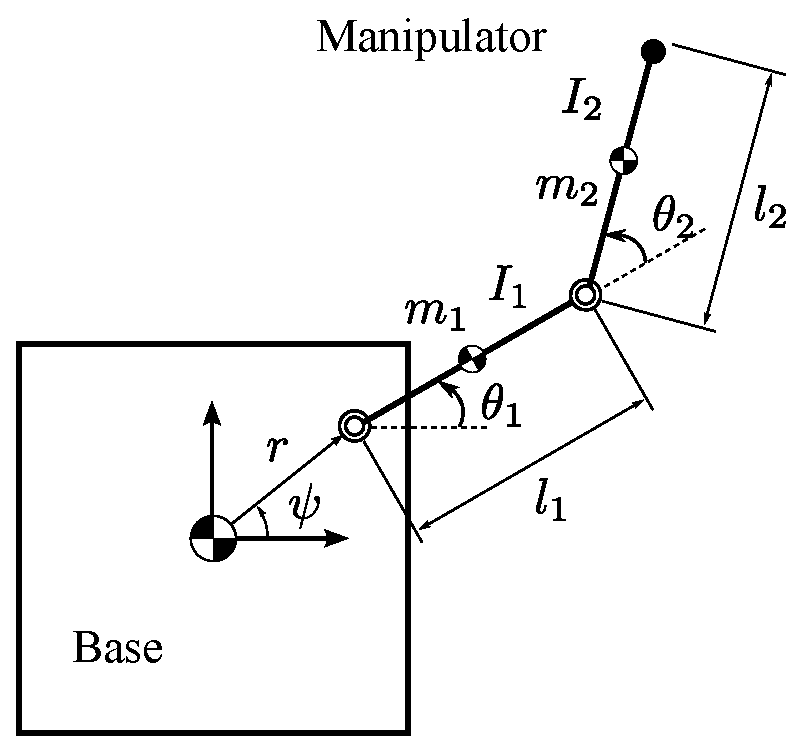
\includegraphics[width=1.0\linewidth]{fig/analysis/planar/FF2RModel.eps}
  \end{minipage}
  \hspace{4mm}
  \begin{minipage}[t]{0.30\linewidth}
    \centering
    \includegraphics[width=1.0\linewidth]{fig/analysis/planar/vectorField.eps}
  \end{minipage}
  \caption{A planar two-DoF space manipulator model with $m_{i} = 100\unit{kg}$,
  $l_{i} = 1.0\unit{m}$ ($i = 1, 2$); the base mass is $m_{b} = 1000\unit{kg}$.
  The vector field is obtain with $r = 0\unit{m}$.}
  \label{fig:FF2R}
\end{figure}
% ---------------------------------------------------------------------
%
Despite there are some results based on reactionless motion control,
the characters of reactionless motion have not been mentioned in pre-reported results.
Here, we describe some details of reactionless motion with a planar model.

We consider a planar two-DoF manipulator as shown in \fig{FF2R}.
This model is the most simplest model which can generate reactionless motion.
Reactionless motion with this model can be represented as follows:
%
% ---------------------------------------------------------------------
\begin{align}
  \thd = b\bm{n}(\th)\label{eq:RNSSYST}
\end{align}
% ---------------------------------------------------------------------
%
where, $\bm{n}(\th)\R{2}$ is the null-space vector of the coupling inertia matrix,
$b$ is an arbitrary scalar.
$\bm{n}(\th)$ can be uniquely obtained through appropriate methods,
i.e.\ Singular Value Decomposition (SVD) or co-factor method.
We assume that $\bm{n}(\th)$ is already normalized,
and $b$ is a time-independent constant scalar, for the sake of simplicity.
Hence, \eq{RNSSYST} can be regarded as an autonomous nonlinear system.
The right hand side in \eq{RNSSYST} defines the vector field of reactionless motion
on the joint space.

We examine the characters of reactionless motion with vector field of the above system.
For the sake of simplicity,
we assume that the manipulator is attached on the CoM of the base.
The masses are $m_{b} = 1000\unit{kg}$, $m_{1} = m_{2} = 100\unit{kg}$,
and the link length are $l_{1} = l_{2} = 1.0\unit{m}$, respectively.
Then, the vector field is depicted in \fig{FF2R}.

Because the manipulator is attached symmetrically,
the vector field has rotational symmetry w.r.t.\ joint 1.
As an important character,
we can see that the reactionless motion is almost composed of the motion of joint 2.
Because reactionless motion is a motion which conserves the angular momentum to zero (or constant),
joints which induce a large angular momentum cannot move widely.
With this model,
the angular momentum induced by the joint 1 motion must be larger than
that of the joint 2 motion due to the large inertia moment and the long moment arm. 
As a result, the above mentioned character is observed.

%%%%%%%%%%%%%%%%%%%%%%%%%%%%%%%%%%%%%%%%%%%%%%%
\subsection{Fixed point and bifurcation}
\label{sec:ANALYSIS_FIXED}
%%%%%%%%%%%%%%%%%%%%%%%%%%%%%%%%%%%%%%%%%%%%%%%
In the above case,
the system does not have fixed points.
However, with variation of a specific parameter,
we can observe occurrence of bifurcation in reactionless motion.
This bifurcation phenomenon is largely related to the manipulator attachment position.
The attachment position is defined as follows:
%
% ---------------------------------------------------------------------
\begin{align}
  \begin{bmatrix}
    x_{a}\\
    y_{a}
  \end{bmatrix}
  =
  r
  \begin{bmatrix}
    \cos\psi\\
    \sin\psi
  \end{bmatrix}
\end{align}
% ---------------------------------------------------------------------
%
where, $(\circ)_{a}$ is the coordinate of the attachment position,
$r$ is the distance between the attachment position and the base CoM,
$\psi$ is the angle as shown in \fig{FF2R}.
Among these parameters, $r$ plays an important role as a \textit{bifurcation parameter} in this system.
Note that we assume $\psi = 0\unit{rad}$ because this parameter does not influence the topological structure
in the system due to rotational symmetry of mechanics.
The condition $\psi = 0\unit{rad}$ means the manipulator
attachment position varies along $x$-axis of the base frame.

%
% --------------------------------------------------------------------
\begin{figure}[t]
  \centering
  \begin{minipage}[t]{0.30\linewidth}
    \centering
    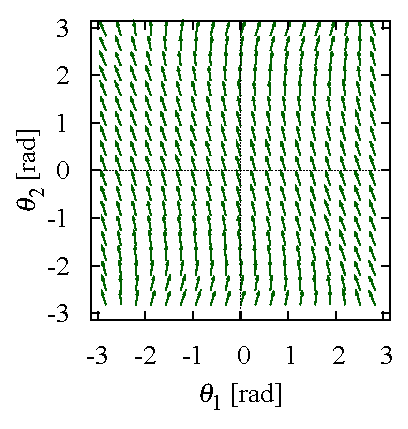
\includegraphics[width=1.0\linewidth]{fig/analysis/planar/0.5.eps}
    \hspace{2mm}
  \end{minipage}
  \begin{minipage}[t]{0.30\linewidth}
    \centering
    \includegraphics[width=1.0\linewidth]{fig/analysis/planar/0.945.eps}
    \hspace{2mm}
  \end{minipage}
  \begin{minipage}[t]{0.30\linewidth}
    \centering
    \includegraphics[width=1.0\linewidth]{fig/analysis/planar/1.5.eps}
    \hspace{2mm}
  \end{minipage}\\
  \vspace{-3mm}
  \begin{minipage}[t]{0.30\linewidth}
    \centering
    \includegraphics[width=1.0\linewidth]{fig/analysis/planar/0.5_nullclines.eps}
    \footnotesize\par{(a)}
    \hspace{2mm}
  \end{minipage}
  \begin{minipage}[t]{0.30\linewidth}
    \centering
    \includegraphics[width=1.0\linewidth]{fig/analysis/planar/0.945_nullclines.eps}
    \footnotesize\par{(b)}
    \hspace{2mm}
  \end{minipage}
  \begin{minipage}[t]{0.30\linewidth}
    \centering
    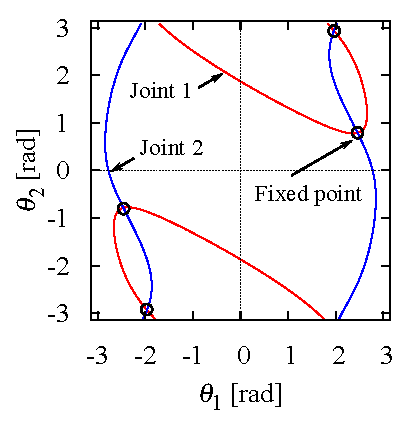
\includegraphics[width=1.0\linewidth]{fig/analysis/planar/1.5_nullclines.eps}
    \footnotesize\par{(c)}
    \hspace{2mm}
  \end{minipage}
  \caption{The vector field and nullclines for each joint direction with variation $r$:
    (a) $r = 0.5\unit{m}$, (b) $r = 0.945\unit{m}$ and (c) $r = 1.5\unit{m}$.}
    \label{fig:BIF_VEC}
\end{figure}
% --------------------------------------------------------------------
%
We show the vector field and nullclines with several values of $r$ in \fig{BIF_VEC}.
In the figures,
the upper part represents the vector field and
the lower part depicts nullclines for each joint direction:
lines in red are nullcline for joint 1, lines in blue are that for joint 2. 
When $r = 0.5\unit{m}$,
we can see that there is no fixed point,
because the motion of joint 2 never stops at any points in joint space.
On the other hand,
occurrence of the bifurcation can be observed when $r \approx 0.945\unit{m}$.
Then, two fixed point are created at intersection points of two nullclines.
Increasing the bifurcation parameter,
the fixed points which were created at same point is gradually separated each other
($r = 1.5\unit{m}$).
Finally, when $r \rightarrow \infty$ two of the fixed points converge to
$\theta_{2} \rightarrow 0\unit{rad}$ and
the others are to be $\theta_{2} \rightarrow \pm\pi\unit{rad}$, respectively.




%%%%%%%%%%%%%%%%%%%%%%%%%%%%%%%%%%%%%%%%%%%%%%%%%%%%%%%%%%%%%%%%
\subsection{The singularities within the coupling inertia matrix}
\label{sec:ANALYSIS_SING}
%%%%%%%%%%%%%%%%%%%%%%%%%%%%%%%%%%%%%%%%%%%%%%%%%%%%%%%%%%%%%%%%
In above discussion,
we showed the existence of the fixed point of reactionless motion control.
This is related to the singularities of the coupling inertia matrix.
In contrast to kinematic singularities,
the singularities of the coupling inertia matrix have not been discussed, so far.
We provide an insight of this singularity with the planar model mentioned above.

%
% ---------------------------------------------------------------------
\begin{figure}[t]
  \centering
  \begin{minipage}[t]{0.42\linewidth}
    \centering
    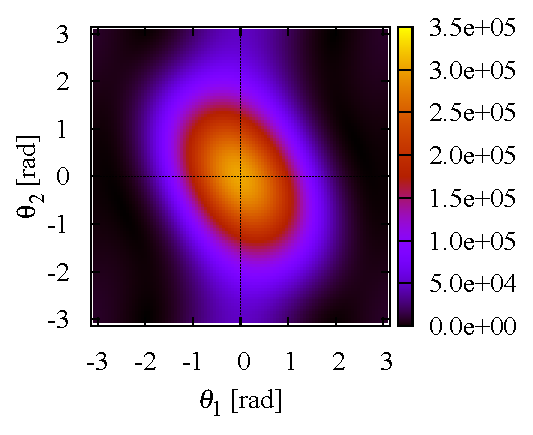
\includegraphics[width=1.0\linewidth]{fig/analysis/planar/determinant.eps}
    \footnotesize\par{(a)}
  \end{minipage}
  \hspace{1mm}
  \begin{minipage}[t]{0.38\linewidth}
    \centering
    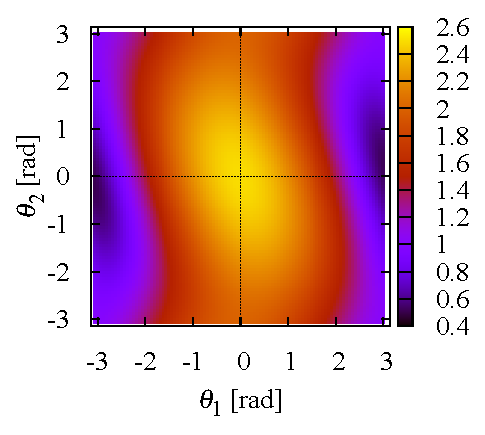
\includegraphics[width=1.0\linewidth]{fig/analysis/planar/com.eps}
    \footnotesize\par{(b)}
  \end{minipage}
  \caption{This figure shows the determinant of the coupling inertia matrix and
  the distance between the manipulator CoM and the base one as color map:
  (a) $\mathrm{det}(\tbm{M}_{\omega m}\tbm{M}_{\omega m})$ and (b) the distance between the manipulator CoM and the base one.}
  \label{fig:DET_FF2R}
\end{figure}
% ---------------------------------------------------------------------
%
We show the determinant of the coupling inertia matrix 
with $r = 1.5\unit{m}$ as a color map in \fig{DET_FF2R}~(a).
In the color map, the determinant takes large values in bright areas, 
while the most dark area represents the singularity.
We can see that the determinant takes its maximum value at $\th = [0~0]^{T}\unit{rad}$.
This is an extended configuration and the manipulator CoM is located on
the farthest away from the base CoM with this configuration.
The determinant of the coupling inertia matrix can be discussed associated with the
distance between the manipulator CoM and the base one,
because the distance determines the amplitude of the coupling angular momentum.
The distance on the joint space is depicted in \fig{DET_FF2R}~(b).
With comparison to these maps,
it can be seen that the determinant takes large values when the distance is long:
there is no fixed point within the location where the CoM distance becomes large.
In the case of spatial models,
the direction of each joint axis become significant,
in addition to this character.


%%%%%%%%%%%%%%%%%%%%%%%%%%%%%%%%%%%%%%%%%%%%%%%%%%%%%%%%%%%%%%%%%%%%%%%%%
\section{Reactionless inspection task using a hand camera}
\label{sec:PROPOSAL}
%%%%%%%%%%%%%%%%%%%%%%%%%%%%%%%%%%%%%%%%%%%%%%%%%%%%%%%%%%%%%%%%%%%%%%%%%
In this section, we will introduce a practical task suitable for execution under
reactionless motion control with a spatial redundant manipulator.
First, we describe the manipulator model and its reactionless motion.
Then, the task description and the control command will be mentioned.
Finally, we verify the performance of the proposed reactionless
task compared with a conventional kinematic controller.


%%%%%%%%%%%%%%%%%%%%%%%%%%%%%%%%%%%%%%%%%%%%%%%%
\subsection{Manipulator model and its reactionless motion}
%%%%%%%%%%%%%%%%%%%%%%%%%%%%%%%%%%%%%%%%%%%%%%%%
%
% ---------------------------------------------------------------------
\begin{figure}[t]
  \centering
  \begin{minipage}[t]{0.65\linewidth}
      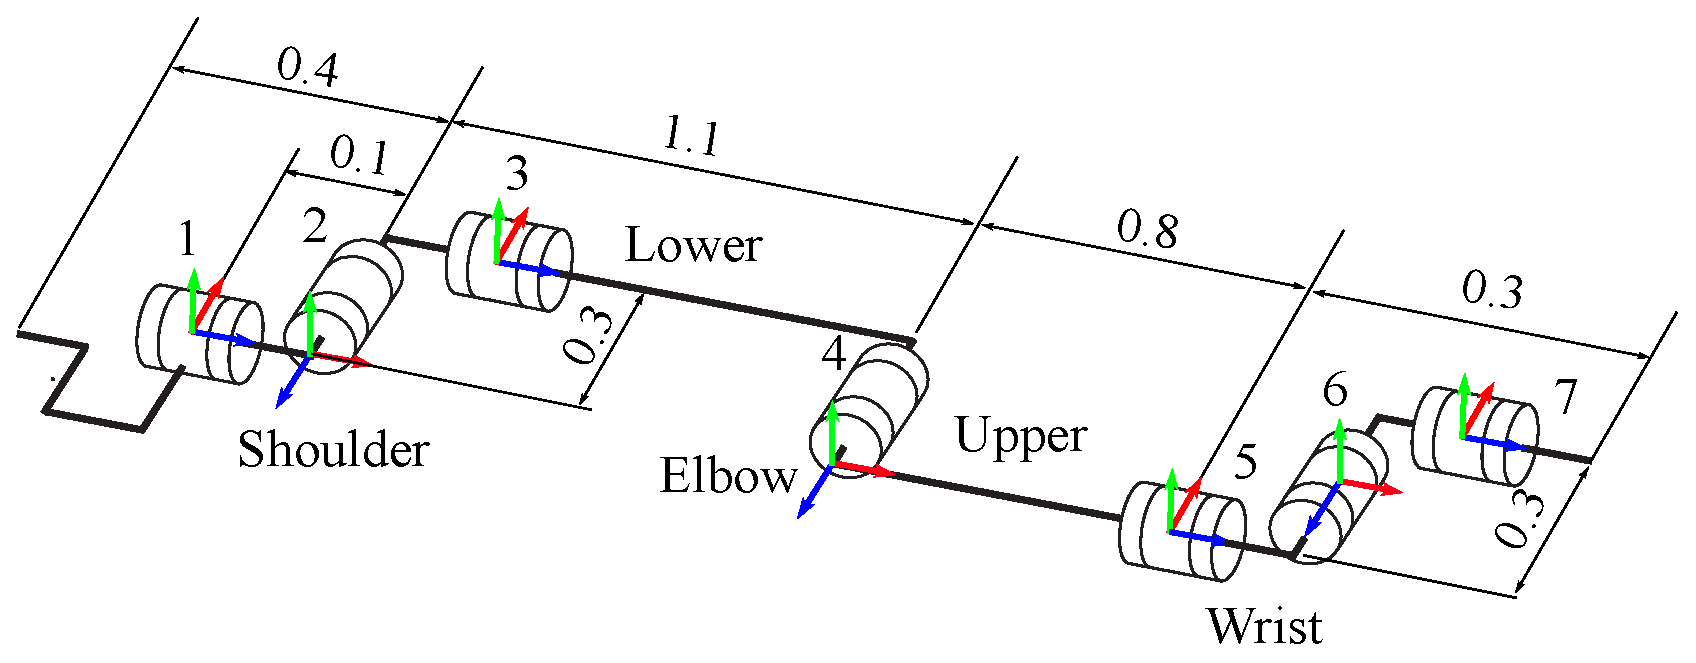
\includegraphics[width=1.0\linewidth]{fig/typeA_7R.eps}
  \end{minipage}
  \begin{minipage}[t]{0.24\linewidth}
    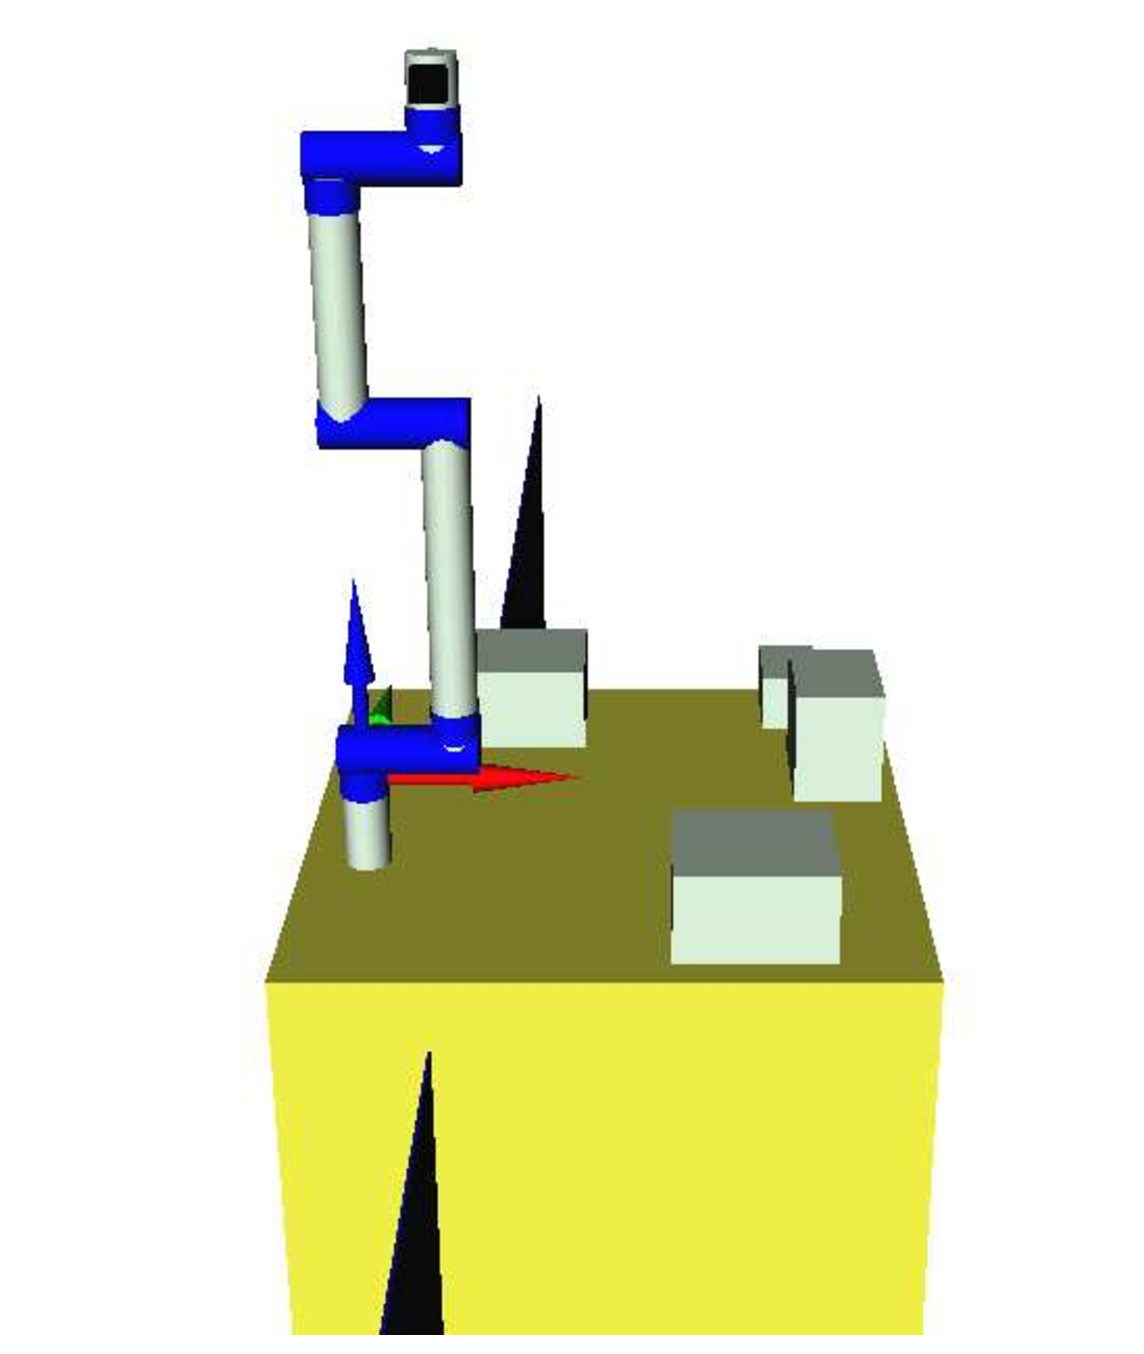
\includegraphics[width=1.0\linewidth]{fig/init.eps}
  \end{minipage}
  \caption{Our manipulator model with seven-DoF mechanism at
    the initial configuration ($\theta_{i} = 0\unit{rad}$, $\forall \theta_{i}$).}
  \label{fig:MODEL}
\end{figure}
% ---------------------------------------------------------------------
%
In this study,
we consider a free-flying space robot model consisting of a satellite base,
a serial seven-DoF redundant manipulator.
The manipulator is characterized by a kinematic chain with a distinctive lower/upper arm
subchain, including a rotational ``elbow'' joint and ``shoulder'' and ``wrist'' joints with offsets.
The kinematic structure and simulation model are displayed in \fig{MODEL}.
The manipulator attachment position are designed based on that of ETS-VII as $[-0.79~-0.29~1.0]^{T}\unit{m}$
with respect to the base CoM \cite{Yoshida2003}.
The dynamic model parameters are shown in \tab{parameter}.
% The reaction wheels are modeled with $10\unit{kg}$ mass and $0.11\unit{kgm^{2}}$ moment of inertia.
%
% ---------------------------------------------------------------------
\begin{table}[t]
  \centering
  \caption{Dynamic model parameters}
  \begin{tabular}[t]{c||c|c|c|c}\hline\hline
    & Mass [kg]&
    \multicolumn{3}{ c }{Inertia moment [$\mathrm{kgm^{2}}$]}\\\hline
    $i$ & $m_{i}$&  $I_{xi}$ & $I_{yi}$ & $I_{zi}$ \\\hline\hline
    $b$ & 2552 & 6200 & 3540 & 7090 \\\hline
    1 & 30.0 & 0.0671 & 0.0671& 0.0851\\\hline
    2 & 30.0 & 0.0843& 0.267 & 0.267\\\hline
    3 & 45.0 & 3.81 & 3.81& 0.127 \\\hline
    4 & 40.0 & 0.113& 2.19 & 2.19\\\hline
    5 & 20.0 & 0.213 & 0.213 & 0.0250\\\hline
    6 & 20.0 & 0.0250 & 0.0292 & 0.0292\\\hline
    7 & 25.0 & 0.0990& 0.0990 & 0.0313\\\hline
  \end{tabular}
  \label{tab:parameter}
\end{table}
% ---------------------------------------------------------------------
%

Before proceeding with the proposal of practical reactionless motion task,
we have to identify reactionless motion with the manipulator model.
In this model,
the DoF of reactionless motion is four,
which is obtained as the difference between the joint number
and the base attitude DoF (three).
The following discussion provides a useful representation of the four-DoF motion.

First,
we divide the kinematic structure into the positioning and the wrist subchains for practical aspect.
The positioning subchain consists of Joint 1 through 4.
The rest of joints constitute the wrist subchain.

Here, we focus on the amplitude of the angular momentum produced by each subchain.
Because of small mass and the length of moment arm,
we can regard that the angular momentum produced by the motion of wrist subchain is far smaller than these of the positioning subchain.
Hence,
it can be considered that the positioning subchain can compensate the base disturbance induced by 
the wrist subchain motion, completely.
% This motion consists of free WS motion and small PS motion
In other words,
a part of the reactionless motion consists of free wrist subchain motions and
small positioning subchain motions as shown in \fig{motion}~(a).
This motion is three-DoF reactionless motion and is defined as
the predominant wrist motion, hereafter.
%
% ---------------------------------------------------------------------
\begin{figure}[t]
  \centering
  \begin{minipage}[h]{0.4\linewidth}
    \centering
    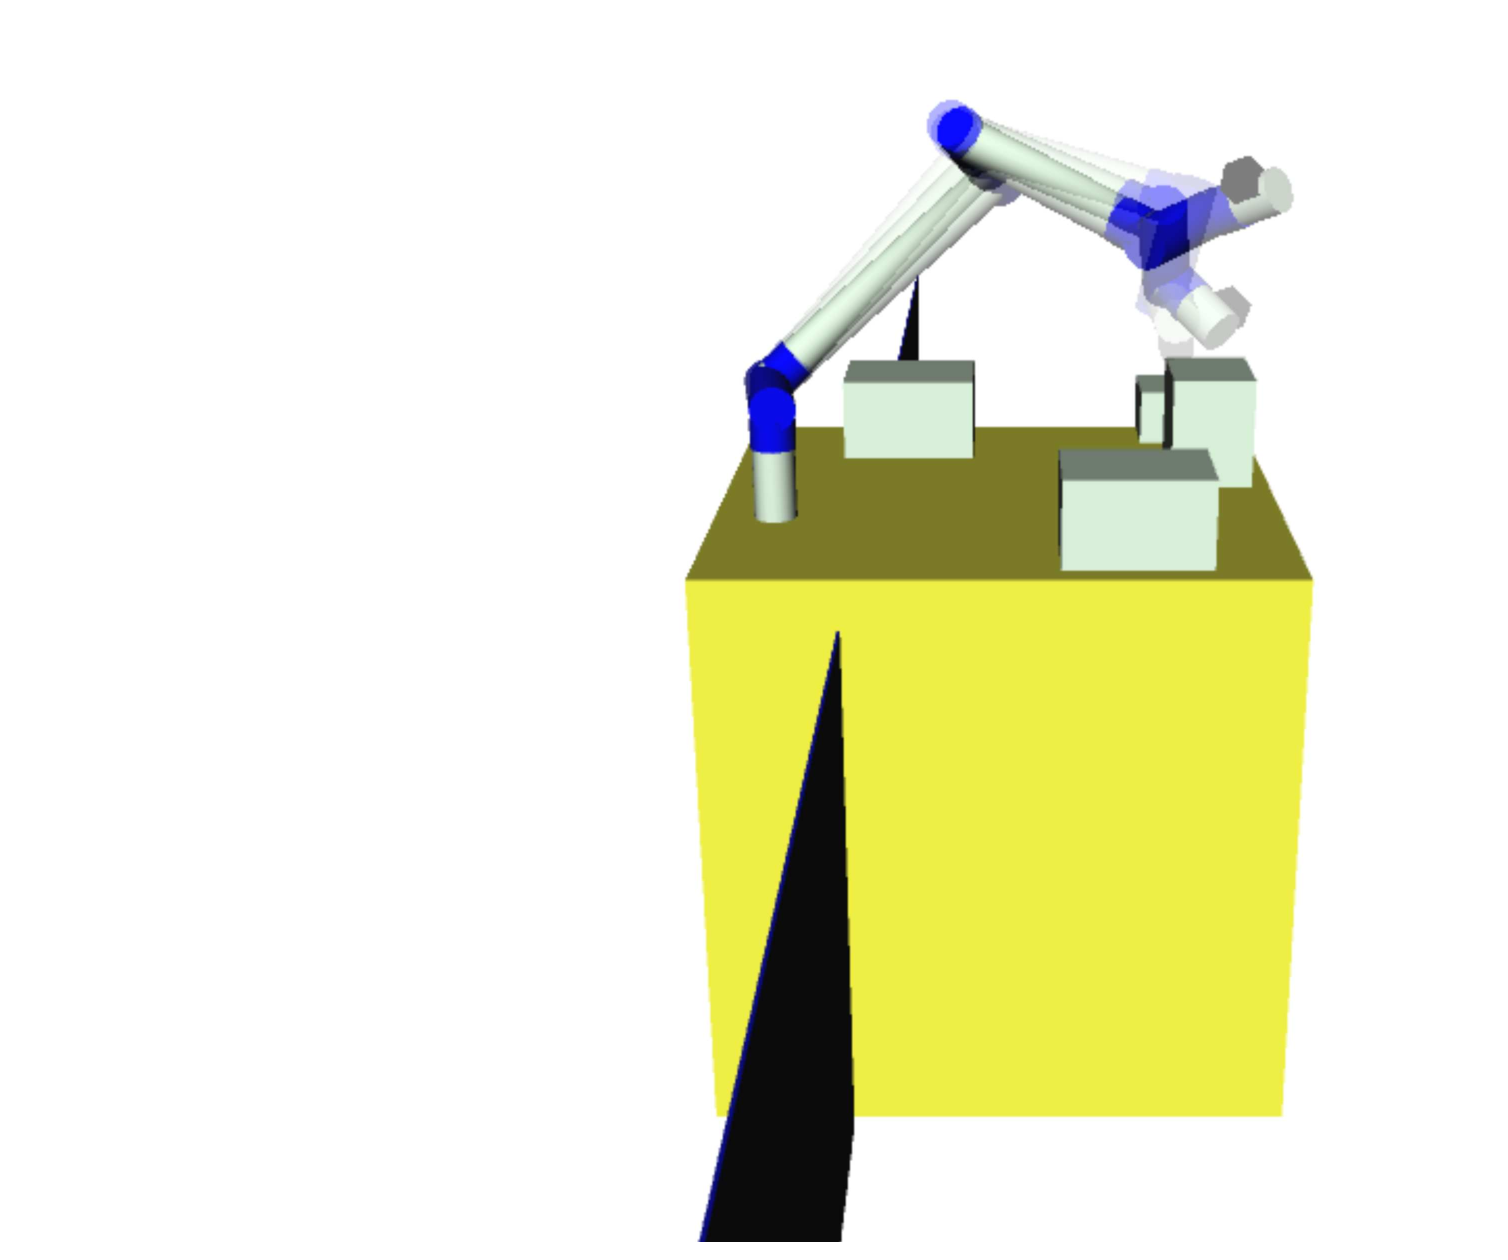
\includegraphics[width=1.0\linewidth]{fig/analysis/WS.eps}
    \footnotesize\par{(a)}
  \end{minipage}
  \begin{minipage}[h]{0.4\linewidth}
    \centering
    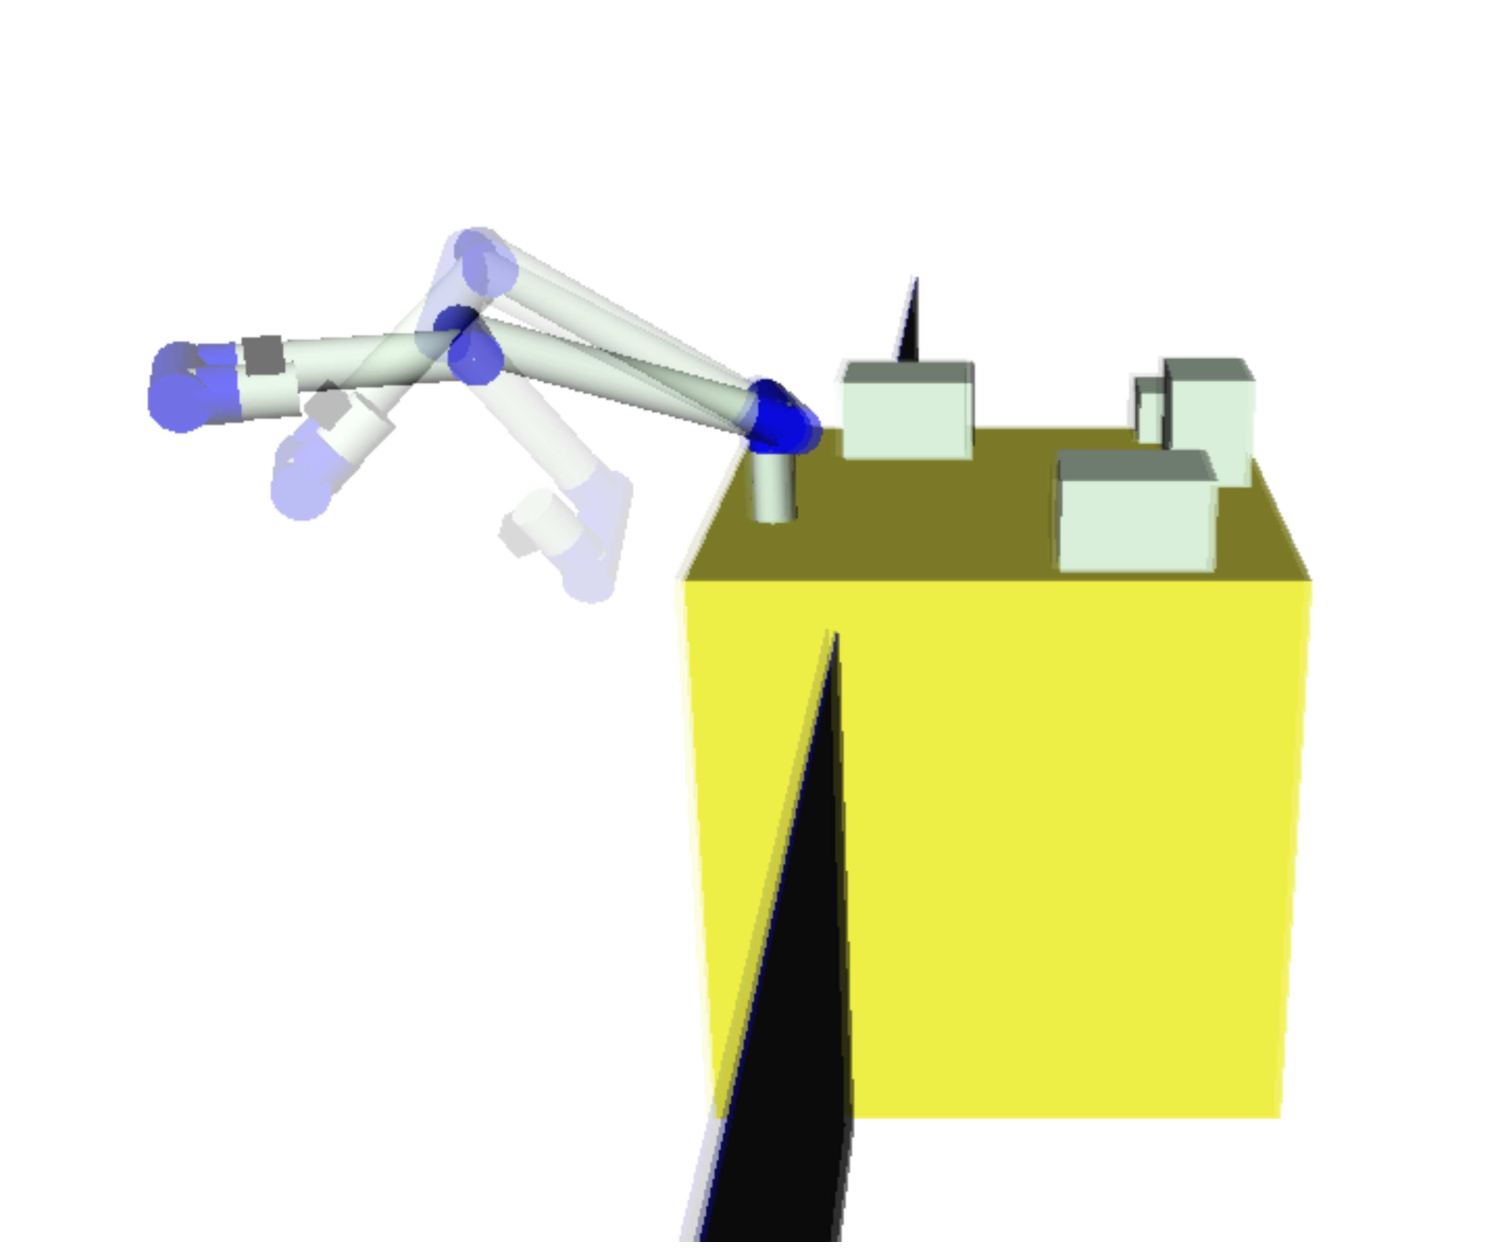
\includegraphics[width=1.0\linewidth]{fig/analysis/PS.eps}
    \footnotesize\par{(b)}
  \end{minipage}
  \caption{Reactionless motion of the manipulator model: (a) the predominant wrist motion and (b) the elbow folding motion.}
  \label{fig:motion}
\end{figure}
% ---------------------------------------------------------------------
%

The remaining one-DoF reactionless motion is uniquely determined as the null-space 
of the submatrix of the coupling inertia matrix related to the positioning subchain part.
This motion approximately consists of the elbow folding/unfolding motion as shown in \fig{motion}~(b).
From angular momentum conservation,
we can assume that the motion of Joint 1 and 2 are relatively small in the above two motions.
Since these two motion are mathematically orthogonal,
the reactionless motion of the our manipulator model can be represented as
the superposition of these motions.

% These motions are represented as follows:
% %
% % ---------------------------------------------------------------------
% \begin{align}
%   \thd &= \bmat{\bm{B}(\th) \\ \bm{E}}\thd_{w} + b \bmat{\bm{n}(\th) \\ \bm{0}}\\
%   \bm{B}(\th) &= -\tbm{M}_{\omega m,P}^{+}\tbm{M}_{\omega m, W}\label{eq:motion}
% \end{align}
% % ---------------------------------------------------------------------
% %
% where,
% $\thd_{w}\R{3}$ stands for the joint velocity of the wrist subchain,
% $\bm{B}(\th)\R{4 \times 3}$ is a linear map from the wrist subchain's disturbance to 
% the joint velocity of the positioning subchain.
% $\tbm{M}_{\omega m,P}\R{3 \times 4}$,
% $\tbm{M}_{\omega m,W}\R{3\times 4}$ are submatrices of the coupling inertia matrix
% related to the positioning and wrist subchain, respectively.
% $\bm{n}\R{4}$ is the uniquely determined null-space vector of $\tbm{M}_{\omega m,P}$.
% This vector can be obtained as co-factor of $\tbm{M}_{\omega m,P}$ or using SVD.
% $b$ is an arbitrary scalar, 
% $\bm{E}\R{3\times 3}$ and $\bm{0}\R{3}$
% denote the identity matrix and zero matrix, respectively.

% In the above equation,
% the first term on the r.h.s.\ represents the predominant wrist motion;
% the second term represents the approximate elbow folding/unfolding motion.
% It should be noted that these motions have orthogonal property 
% because of $\bm{B}^{T}\bm{n} = \bm{0}$.
% Hence it is apparent that reactionless motion of the model
% is represented as superposition of these motions.

From the above analysis, we can obtain the following fact:
because the end-effector position largely depends on the motion of the positioning subchain,
the DoF of the end-effector position control under reactionless motion
is approximately 1 according to that of the positioning subchain.
Namely, even if the system has enough DoF,
position control under reactionless motion is not feasible due to the limitation of
the kinematic structure.
From the reason,
we focus on the end-effector orientation control with the predominant wrist motion
rather than considering the position control.
This makes our research different from the previous studies.


%%%%%%%%%%%%%%%%%%%%%%%%%%%%%%%%%%
\subsection{Reactionless inspection task}
\label{sec:INSPECTION}
%%%%%%%%%%%%%%%%%%%%%%%%%%%%%%%%%%
%%%%%%%%%%%%%%%%%%%%%%%%%%%%%%%%%%
\subsubsection{Task definition}
\label{sec:MISSION}
%%%%%%%%%%%%%%%%%%%%%%%%%%%%%%%%%%

%
% ---------------------------------------------------------------------
\begin{figure}[t]
  \centering
  \begin{minipage}[h]{0.495\linewidth}
    \centering
    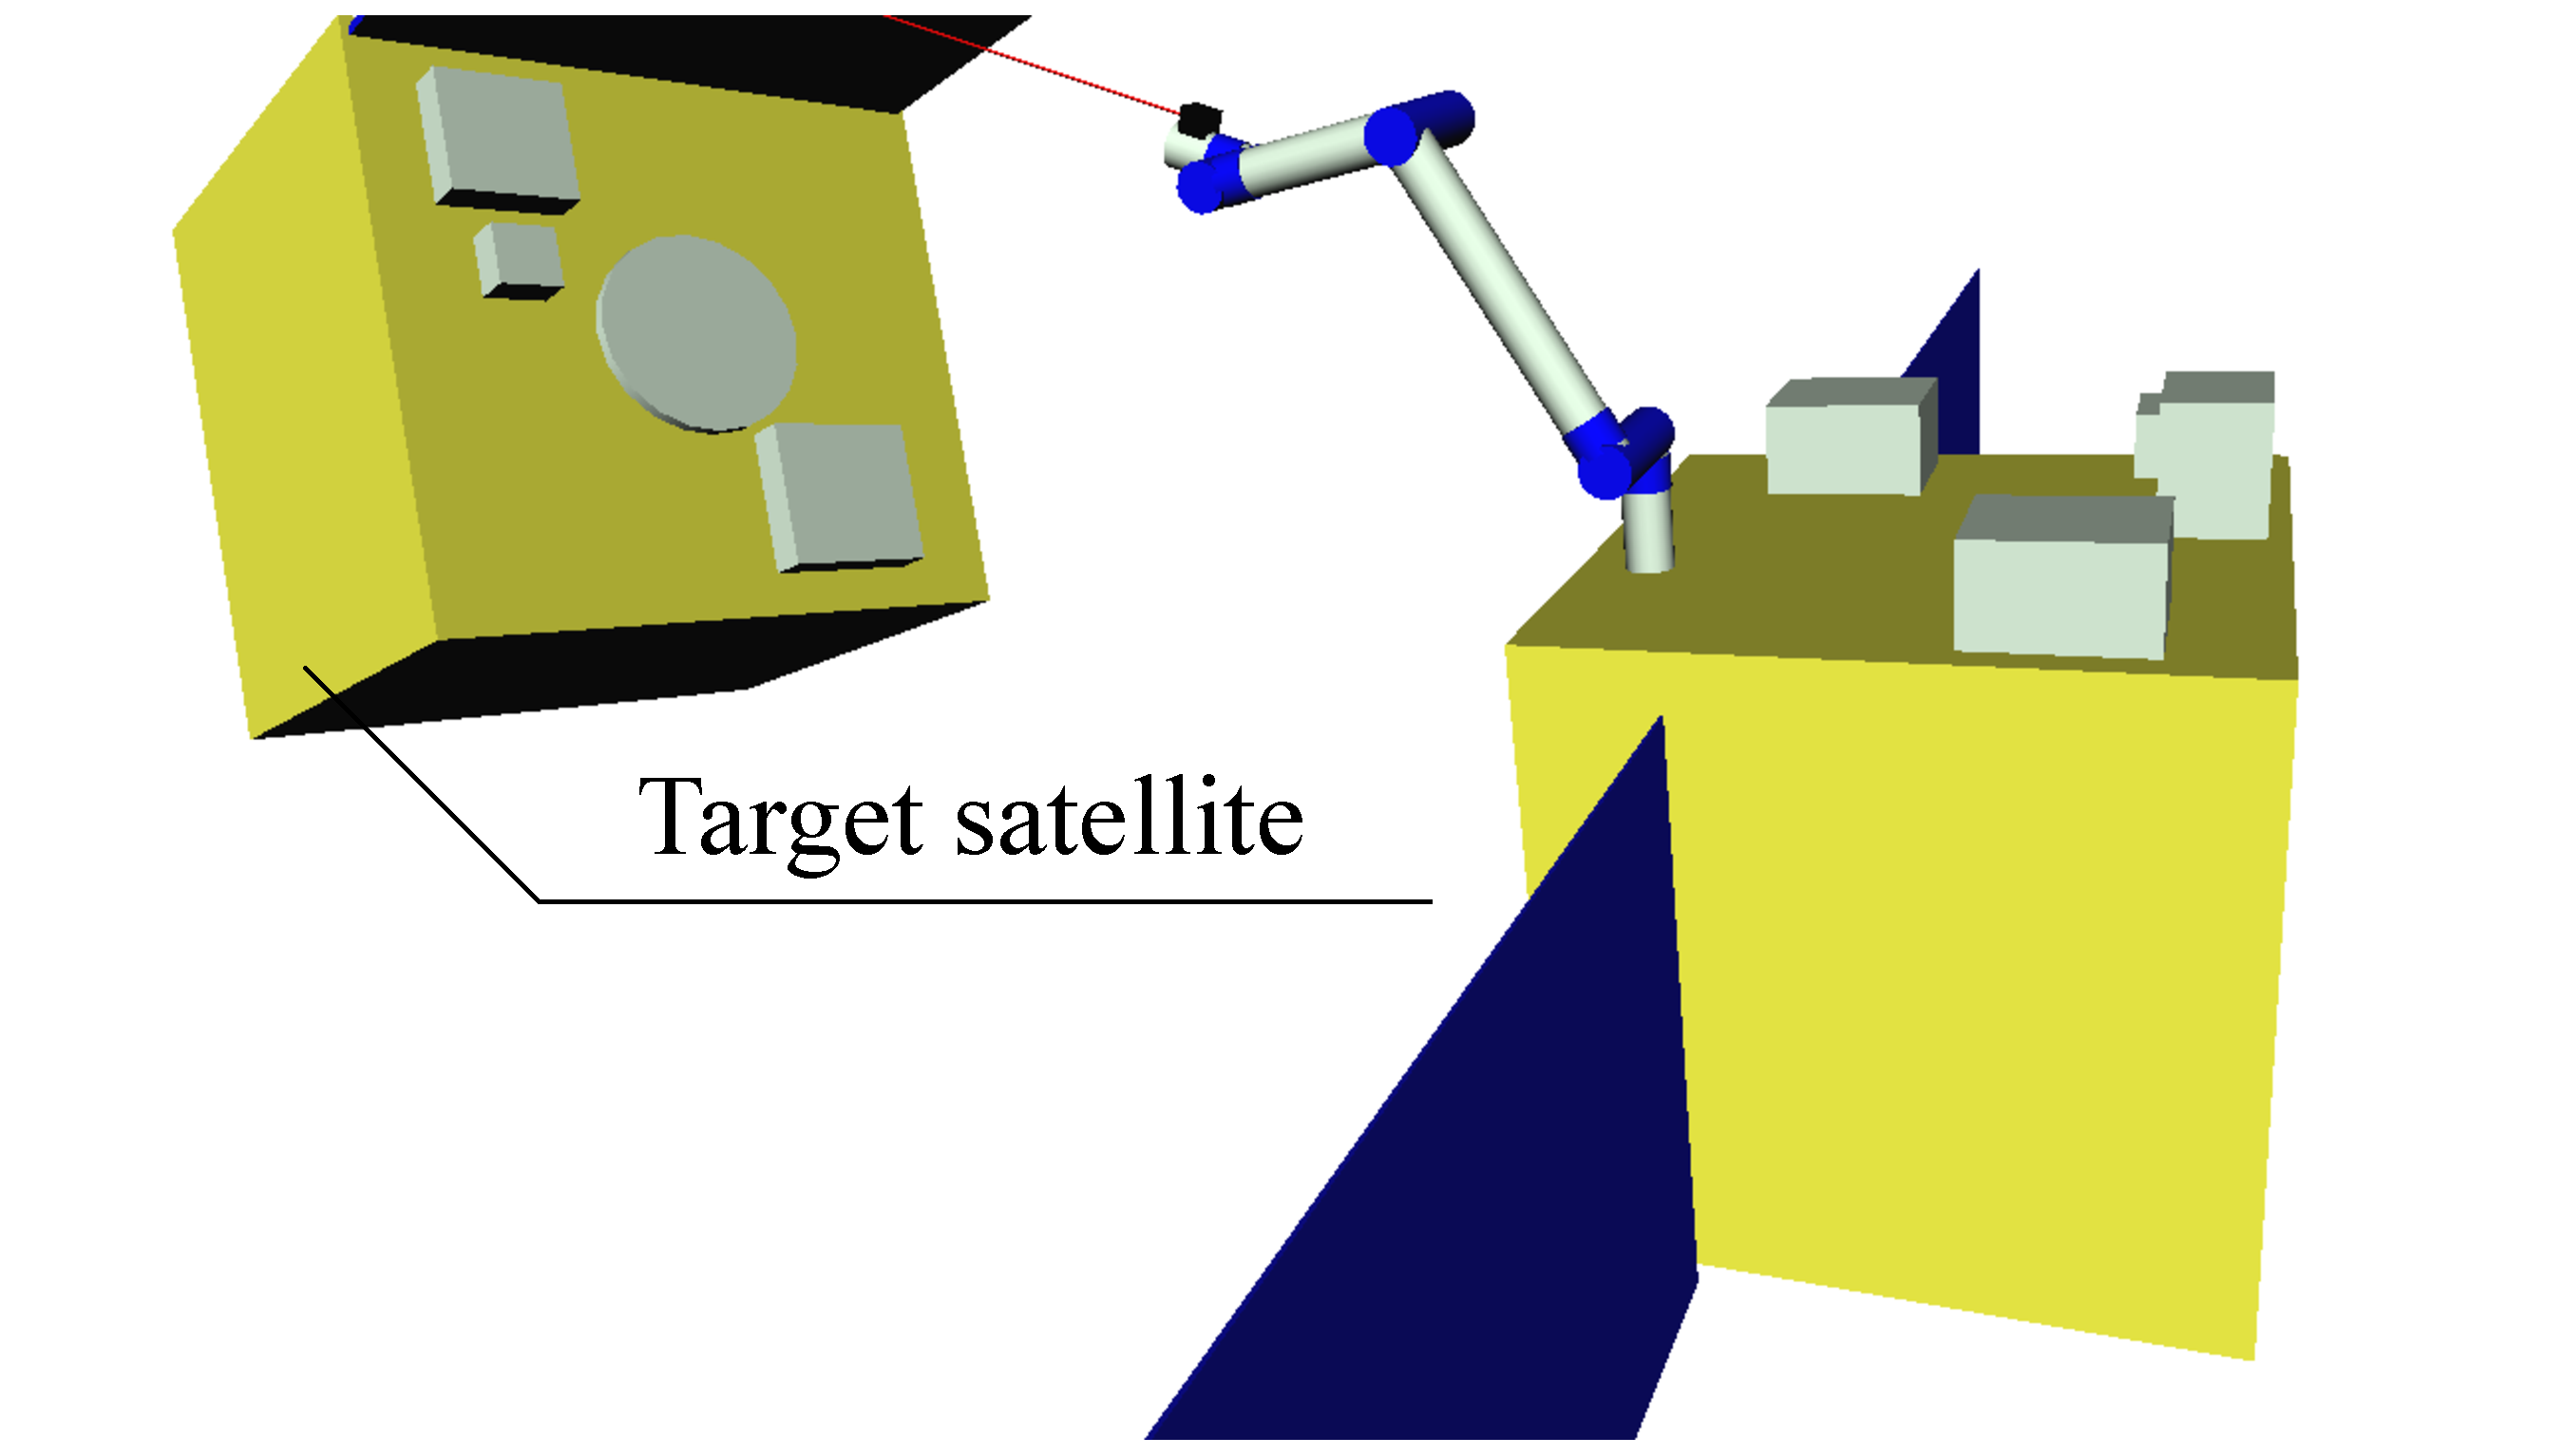
\includegraphics[width=1.0\linewidth]{fig/proposal/inspection/observation.eps}
    \footnotesize\par{(a)}
  \end{minipage}
  \begin{minipage}[h]{0.495\linewidth}
    \centering
    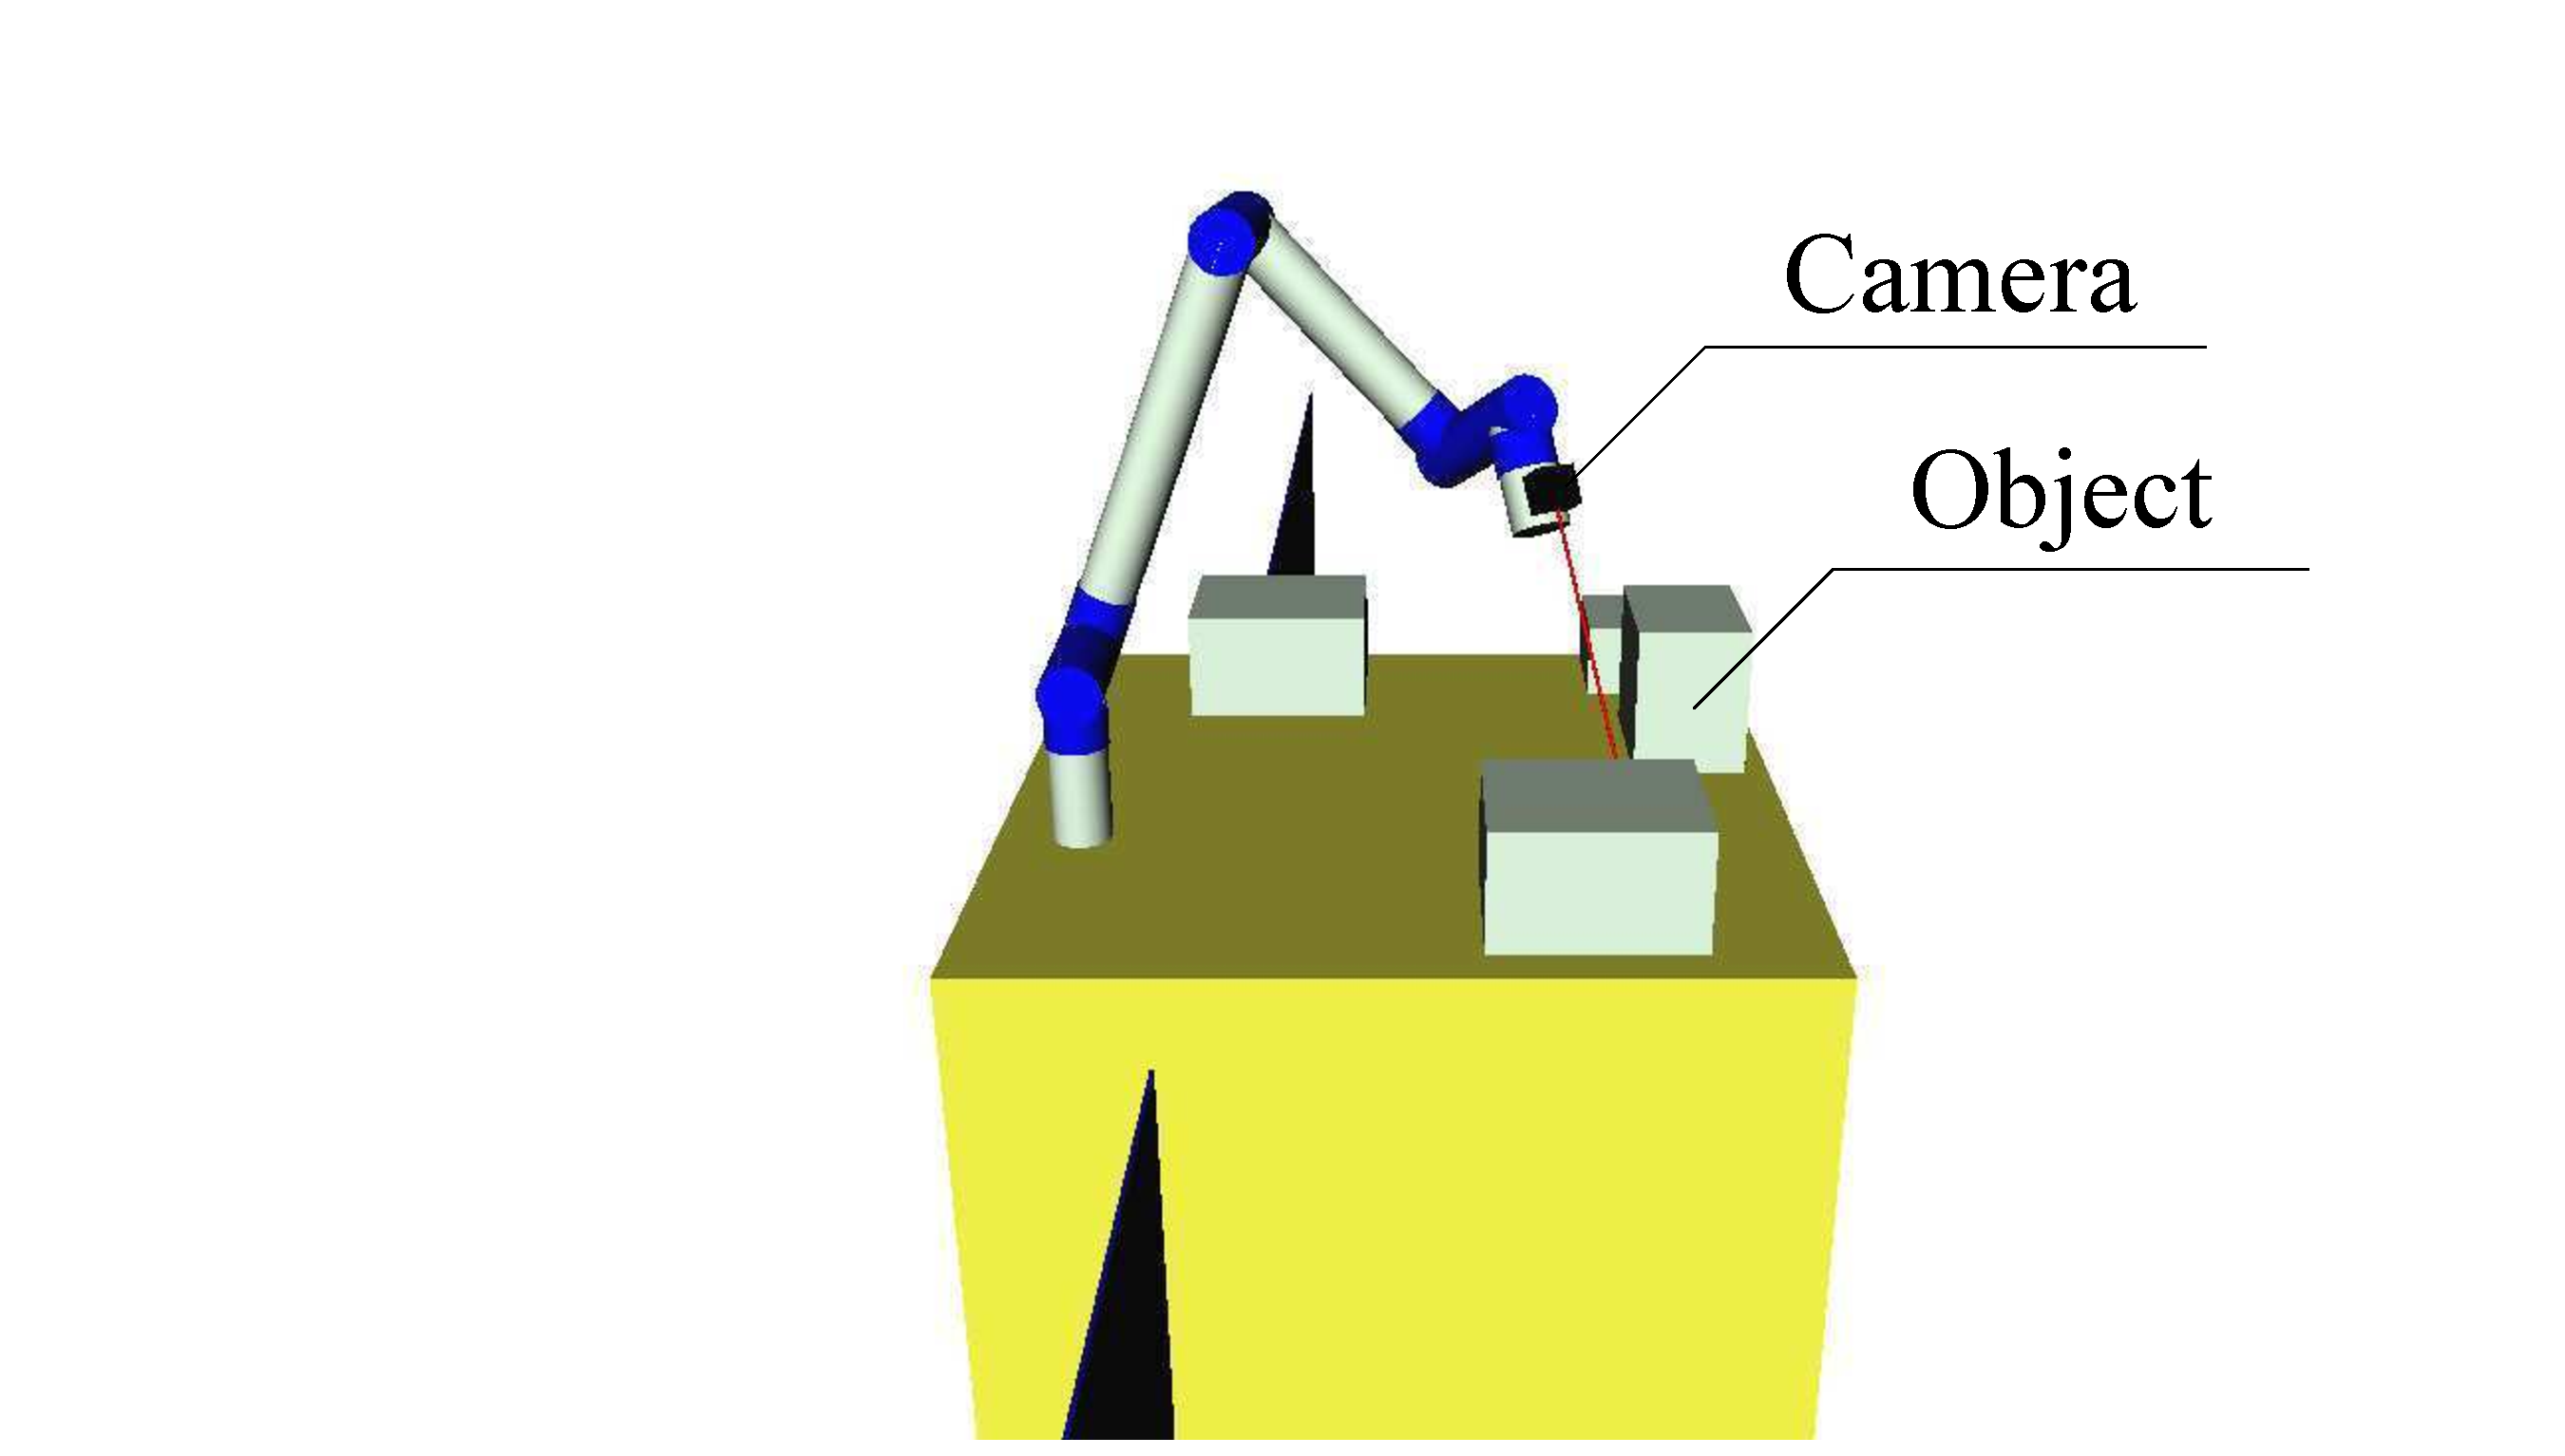
\includegraphics[width=1.0\linewidth]{fig/proposal/inspection/inspection.eps}
    \footnotesize\par{(b)}
  \end{minipage}
  \caption{Inspection task using the hand camera: 
    (a) target satellite to be refueled of captured and (b) own-satellite attached devices.}
  \label{fig:ins}
\end{figure}
% ---------------------------------------------------------------------
%
One frequent task for free-floating space robots is inspection with a hand camera for various devices mounted
on own satellite, large space structures or satellites to be serviced, as shown in \fig{ins}.
Such task was also performed within the ETS-VII mission \cite{Oda1997} without using reactionless control.
At this motion task, once the arm is positioned appropriately,
the camera view angle for inspection is changed by rotating the wrist.
This task would be expected to perform several times in almost all kind of missions,
such as construction, maintenance, debris removal and so on.
Hence, this task is a good candidate for execution under reactionless motion control
to reduce work efficiency.

We consider the following three tasks in order to accomplish the camera inspection.
%
% ---------------------------------------------------------------------
\begin{enumerate}
\item Reactionless constraint of the base attitude (three-DoF)
\item Orientation control of the end-effector (three-DoF)
\item Stabilization of the wrist position
\end{enumerate}
% ---------------------------------------------------------------------
%
The third one is due to the following reason:
a large deflection of the wrist
might induce a collision problem and camera view changes.

The above tasks are simultaneously realized through the theory of task priority \cite{Nakamura1987}.
In this theory,
the tasks are assigned the priorities according to its relative importance.
The highest priority task, which is called the \textit{primary task}, can be accomplished
without the effect from lower priority tasks.
Hence, lower priority tasks must be designed not to disturb the higher priority tasks.
% these task can be realized iff the above priority ensures.
In order to unsure the prioritization,
lower priority tasks are projected to the null-space of all-higher priority tasks.
We make a control command according to this theory.

%%%%%%%%%%%%%%%%%%%%%%%%%%%%%%%%%%
\subsubsection{Control command}
\label{sec:CONTROLLER}
%%%%%%%%%%%%%%%%%%%%%%%%%%%%%%%%%%
We regard the reactionless constraint as the primary task,
the end-effector orientation control is the second one and the wrist position stabilization is the third one.
The control command of the joint velocity, considering
the above priorities, can be obtained as follows:
%
% ---------------------------------------------------------------------
\begin{align}
  \thd^{ref} = {}^{e}\bar{\bm{J}}_{\omega}^{+}\bm{\omega}_{e}^{ref} + k_{g}\bm{P}{}^{w}\bm{J}_{v}^{T}\Delta\bm{p}_{w}
  \label{eq:REF}
\end{align}
% ---------------------------------------------------------------------
%
where,
$\bm{\omega}_{e}\R{3}$ is angular velocity of the end-effector,
${}^{e}\bar{\bm{J}}_{\omega} = [{}^{e}\bm{J}_{\omega}\bm{P}_{RNS}]\R{3 \times 7}$ is the restricted Jacobian matrix,
${}^{e}\bm{J}_{\omega}$ and
${}^{w}\bm{J}_{v}\R{3 \times 7}$ stand for the Jacobian w.r.t.\ the angular velocity of the end-effector
and wrist linear velocity.
Superscripts explain the specific point associated with the velocities.
Note that the superscript of the end-effector ${}^{e}(\circ)$ will be ignored for description convenience, hereafter.
% $\bm{P}_{RNS}\R{7 \times 7}$ is the Reaction Null-Space projector described above,
$\bm{P} = \bm{P}_{RNS}(\bm{E} - \bar{\bm{J}}_{\omega}^{+}\bar{\bm{J}}_{\omega})$ projects
an arbitrary vector onto the null-space of the base and the end-effector tasks \cite{Dietrich2015}.
$\Delta\bm{p}_{w} (= \bm{p}_{w} - \bm{p}_{w}^{init})\R{3}$ is the wrist-position deflection from the initial one,
$k_{g}$ is a gradient gain.

The structure of the control command is as follows.
The first term is the end-effector orientation control projected onto the null-space of
the coupling inertia matrix:
this term can accomplish the end-effector orientation control under the reactionless constraint.
The second term minimizes the following potential function to stabilize the wrist position:
%
% ---------------------------------------------------------------------
\begin{align}
 V = \frac{1}{2}\|\Delta\bm{p}_{w}\|^{2}.
\end{align}
% ---------------------------------------------------------------------
%
This term does not disturb the higher priority tasks because it is projected
onto the null-space of all higher priority tasks.

Here, it must be noted that $\bar{\bm{J}}_{\omega}^{+}$ includes the algorithmic singularities,
which occur when the end-effector control and the reactionless constraint are conflict.
The details of this singularity will be described, below.

%%%%%%%%%%%%%%%%%%%%%%%%%%%%%%%%%%
\subsubsection{Numerical simulation}
\label{sec:SIMULATION}
%%%%%%%%%%%%%%%%%%%%%%%%%%%%%%%%%%
In what follows,
we examine the performance under \eq{REF} by comparing to
the following conventional inverse Jacobian controller with motionless of the positioning subchain.
We assume two situations:
(i) observation of a satellite to be serviced (\fig{ins}~(a)) and
(ii) inspection for own satellite mounted devices (\fig{ins}~(b)).

%
% ---------------------------------------------------------------------
\begin{figure}[t]
  \centering
  \begin{minipage}[h]{0.60\linewidth}
    \centering
    \includegraphics[width=1.0\linewidth]{fig/proposal/inspection/case1/joint.eps}
  \end{minipage}\\
  \begin{minipage}[h]{0.40\linewidth}
    \includegraphics[width=1.0\linewidth]{fig/proposal/inspection/case1/RL-M/U01_joint_velo.eps}
  \end{minipage}
  \hspace{-7mm}
  \begin{minipage}[h]{0.40\linewidth}
    \includegraphics[width=1.0\linewidth]{fig/proposal/inspection/case1/CONV/U01_joint_velo.eps}
  \end{minipage}\\
  \vspace{-5mm}
  \begin{minipage}[h]{0.27\linewidth}
    \centering
    \includegraphics[width=1.0\linewidth]{fig/proposal/inspection/case1/cartesian.eps}
  \end{minipage}\\
  \vspace{-2mm}
  \begin{minipage}[h]{0.40\linewidth}
    \includegraphics[width=1.0\linewidth]{fig/proposal/inspection/case1/RL-M/U20_EE_vel_error.eps}
  \end{minipage}
  \hspace{-7mm}
  \begin{minipage}[h]{0.40\linewidth}
    \includegraphics[width=1.0\linewidth]{fig/proposal/inspection/case1/CONV/U20_EE_vel_error.eps}
  \end{minipage}\\
  \vspace{-5mm}
  \begin{minipage}[h]{0.35\linewidth}
    \centering
    \includegraphics[width=1.0\linewidth]{fig/proposal/inspection/case1/orientation.eps}
  \end{minipage}\\
  \vspace{-2mm}
  \begin{minipage}[h]{0.40\linewidth}
    \centering
    \includegraphics[width=1.0\linewidth]{fig/proposal/inspection/case1/RL-M/X02_Base_Orientation.eps}
    \footnotesize\par{\hspace{8mm}\vspace{-2mm}Reactionless}
  \end{minipage}
  \hspace{-7mm}
  \begin{minipage}[h]{0.40\linewidth}
    \centering
    \includegraphics[width=1.0\linewidth]{fig/proposal/inspection/case1/CONV/X02_Base_Orientation.eps}
    \footnotesize\par{\hspace{8mm}\vspace{-2mm}Conventional}
  \end{minipage}
  \vspace{1em}
  \caption{Simulation result under the satellite observation mission (\fig{ins}~(a)).
  The result shows that reactionless task can be accomplished,
while a large base attitude deviation is observed under the conventional control method.}
  \label{fig:RES_INS}
\end{figure}
% ---------------------------------------------------------------------
%
First, we verify the satellite observation case.
The initial configuration is set as $[-90~-30~0~-70~180~-30~0]^{T}\unit{deg}$ as shown in \fig{ins}~(a),
the reference angular velocity is $\bm{\omega}_{e}^{ref} = \pi[s(t)~0~0]^{T}$,
where $0 \leq s(t) \leq 1$ denotes a fifth-order polynomial interpolation.
The simulation was conducted with the simulation time $20\unit{s}$.
The simulation results are displayed in \fig{RES_INS}.
These are obtained with $k_{g} = 100$.
In both methods, it can be seen that the end-effector task is accomplished.
It is also seen that the base attitude deviation is not observed under reactionless motion control.
The reactionless manner can be realized with the relatively small motion of the positioning subchain,
see the figure of joint velocity.
We should note that a relatively large base attitude deviation
\footnote{The limitation of the base attitude deviation is $0.05\unit{deg}$ in the ETS-VII missions.}
is induced under the conventional control method,
despite the low inertia parameters of the wrist.




%
% ---------------------------------------------------------------------
\begin{figure}[t]
  \centering
  \begin{minipage}[h]{0.60\linewidth}
    \centering
    \includegraphics[width=1.0\linewidth]{fig/proposal/inspection/case1/joint.eps}
  \end{minipage}\\
  \begin{minipage}[h]{0.40\linewidth}
    \centering
    \includegraphics[width=1.0\linewidth]{fig/proposal/inspection/case2/RL-M/U01_joint_velo.eps}
  \end{minipage}
  \begin{minipage}[h]{0.40\linewidth}
    \centering
    \includegraphics[width=1.0\linewidth]{fig/proposal/inspection/case2/CONV/U01_joint_velo.eps}
  \end{minipage}\\
  \vspace{-5mm}
  \begin{minipage}[h]{0.40\linewidth}
    \centering
    \includegraphics[width=1.0\linewidth]{fig/proposal/inspection/case2/RL-M/U13_wrist_deflection.eps}
    \footnotesize\par{\hspace{8mm}\vspace{-2mm}Reactionless}
  \end{minipage}
  \begin{minipage}[h]{0.40\linewidth}
    \centering
    \includegraphics[width=1.0\linewidth]{fig/proposal/inspection/case2/CONV/X02_Base_Orientation.eps}
    \footnotesize\par{\hspace{8mm}\vspace{-2mm}Conventional}
  \end{minipage}
  \vspace{1em}
  \caption{Simulation result under the inspection of own-satellite mounted devices (\fig{ins}~(b)).}
  \label{fig:RES_INS2}
\end{figure}
% ---------------------------------------------------------------------
%
In the second case,
we assume that the initial configuration is set to $[90~-20~180~110~0~20~0]^{T}\unit{deg}$ as shown in \fig{ins}~(b),
the desired end-effector velocity is $\bm{\omega}_{e}^{ref} = \pi[0~0~-s(t)]^{T}\unit{rad/s}$.
The other conditions are same as the previous ones.
The simulation result is displayed in \fig{RES_INS2}.
First, it becomes apparent that the effect of the cost function leads to a sufficiently small deviation from
the initial wrist position as shown in \fig{RES_INS2}.
In the case of the conventional controller,
the relatively large base attitude deviation is also confirmed.

In summary,
in the inspection task,
even with the small mass and inertia moment of the wrist subchain,
a large base attitude deviations were observed.
From the results,
we can conclude that this reactionless motion task is a useful way to overcome this problem.
% Therefore, we can conclude that this reactionless task can be used in practice.


%%%%%%%%%%%%%%%%%%%%%%%%%%%%%%%%%%%%%%%%%%%%%%%%%%%%%%%%%
\section{The singularities within the reactionless inspection task}
\label{sec:SINGULAR}
%%%%%%%%%%%%%%%%%%%%%%%%%%%%%%%%%%%%%%%%%%%%%%%%%%%%%%%%%
%%%%%%%%%%%%%%%%%%%%%%%%%%%%%%%%%
\subsection{Problem statement}
\label{sec:PROBLEM}
%%%%%%%%%%%%%%%%%%%%%%%%%%%%%%%%%

In this section, we deal with the singularities within the proposed reactionless task.
Within the reactionless camera inspection,
there are three type of singularities, as follows:
\begin{itemize}
\item Kinematic singularity: $\mathrm{det}(\bm{J}_{\omega}\bm{J}_{\omega}^{T}) = 0$
\item Singularities of the coupling inertia matrix: $\mathrm{det}(\tbm{M}_{\omega m}\tbm{M}_{\omega m}^{T}) = 0$
\item Algorithmic singularities: $\mathrm{det}(\bar{\bm{J}}_{\omega}\bar{\bm{J}}_{\omega}^{T}) = 0$
with non-singular $\bm{J}_{\omega}$ and full row-rank $\tbm{M}_{\omega m}$
\end{itemize}

Among them, kinematic singularities have been much discussed by various researchers, e.g.\ \cite{Kreutz-Delgado1992,Boudreau2010}.
From these results,
the kinematic singularity can be dealt with some singularity treatment techniques.
The most famous one is the damped least-squares inverse (DLS) \cite{Chiaverini1994}.
Using these method, growth up of the joint velocity can be suppressed through adding a damping factor.
A drawback of this method is causing an error on the task space, both speed and direction.
On the other hand, we have proposed another method, which is called the Singularity Consistent method \cite{Nenchev2000}.
Under this method, the manipulator can follow the desired path without causing a large joint velocity
\footnote{The term ``Path'' is distinguished from ``Trajectory'':
the former one means geometrical path and the later one includes time-parameter.}.
In both method,
the feasibility has been verified under the kinematic singularities.
Hence, we will not pay attention this type of singularity below.

On the other hand,
the second and third one have not been treated.
However,
the singularities of the coupling inertia matrix is not a problem,
because we use the null-space of the coupling inertia matrix.
In \eq{REF},
the rank of $\bar{\bm{J}}_{\omega}$ depends on the condition of $\bm{J}_{\omega}$ only,
since the rank of $\bm{P}_{RNS}$ cannot be lower than 3 with any configurations:
e.g.\ at the singular configuration the rank increases more than 4.
Hence, we will not also pay attention this type of singularities.

The algorithmic singularities must be taken into account.
The inversion of $\bar{\bm{J}}_{\omega}$ can be rewritten through SVD in the following form:
%
% ---------------------------------------------------------------------
\begin{align}
  \bar{\bm{J}}_{\omega}^{+} = \frac{1}{\sigma_{1}}\bm{v}_{1}\bm{u}_{1}^{T} + 
  \frac{1}{\sigma_{2}}\bm{v}_{2}\bm{u}_{2}^{T} + 
  \frac{1}{\sigma_{3}}\bm{v}_{3}\bm{u}_{3}^{T}\label{eq:JP_SVD}
\end{align}
% ---------------------------------------------------------------------
%
where, $\sigma_{1} \geq \sigma_{2} \geq \sigma_{3}$ are the singular values,
$\bm{v}_{i}\R{7}$, $\bm{u}_{i}\R{3}$ are the left and right singular vectors
associated with $\sigma_{i}$.
Near the singularities,
the last term of \eq{JP_SVD} takes a large value due to small value of $\sigma_{3}$.

In what follows, we show an example of the algorithmic singularity.
We assume the inspection task with the same initial configuration
which was used in the satellite observation task as shown in \fig{ins}~(a).
On the other hand, the desired angular velocity is commanded as $\bm{\omega}_{e}^{ref} = [0~-0.2~0]^{T}\unit{rad/s}$.
The simulation results are displayed in \fig{RES_SIN}.
%
% ---------------------------------------------------------------------
\begin{figure}[t]
  \centering
  \begin{minipage}[t]{0.40\linewidth}
    \centering
    \includegraphics[width=1.0\linewidth]{fig/proposal/singularity/SAMPLE/U01_joint_velo.eps}
  \end{minipage}
  \begin{minipage}[t]{0.40\linewidth}
    \centering
    \includegraphics[width=1.0\linewidth]{fig/proposal/singularity/SAMPLE/U16_determinant_Gw.eps}
  \end{minipage}\\
  \vspace{-1mm}
  \begin{minipage}[t]{0.40\linewidth}
    \centering
    \includegraphics[width=1.0\linewidth]{fig/proposal/singularity/SAMPLE/U14_determinant_Jw.eps}
  \end{minipage}
  \begin{minipage}[t]{0.40\linewidth}
    \centering
    \includegraphics[width=1.0\linewidth]{fig/proposal/singularity/SAMPLE/U15_determinant_Mwm.eps}
  \end{minipage}
  \caption{An example of the algorithmic singularity within the proposed method.}
  \label{fig:RES_SIN}
\end{figure}
% ---------------------------------------------------------------------
%
In the graphs,
the solid line in black represents the time when
the manipulator is passing through near the singularity ($t \approx 2.57$).
At that time, the determinant of $\bar{\bm{J}}_{\omega}$ takes a small value
without causing $\mathrm{det}(\bm{J}_{\omega}\bm{J}_{\omega}^{T}) = 0$ and
$\mathrm{det}(\tbm{M}_{\omega m}\tbm{M}_{\omega m}^{T}) = 0$ as shown in \fig{RES_SIN}.
Hence, this singularity can be recognized as the algorithmic one.
Within the near singularity,
we observe that joint 5 and 7 rotate around opposite direction with large joint velocity.
This kind of behavior has been observed at the singularity of Euler angle \cite{Taki2013}
and the kinematic singularity of wrist assemblies.

From the empirically obtained results,
this algorithmic type of singularity does not seem to happen frequently.
Besides,
even if the singularity happens,
we will show a well-known singularity treatment technique,
so-called the damped least-squares inverse,
can relieve the influence of the singularity.

%%%%%%%%%%%%%%%%%%%%%%%%%%%%%%%%%%%%%%%%%%%%%%%%%%%%%%%%%%%%%%%%%%%%%%%%%
\subsection{The damped least-squares inverse based singularity treatment}
\label{sec:SIN_DLS}
%%%%%%%%%%%%%%%%%%%%%%%%%%%%%%%%%%%%%%%%%%%%%%%%%%%%%%%%%%%%%%%%%%%%%%%%%
The damped least-squares inverse is a well-known approach for singularity problem.
This method is adding a damping factor into the denominators in \eq{JP_SVD} to avoid
causing a large joint velocity.
Among various types of the damped least-squares inverse,
we use that with numerical filtering because this method does not cause a large error.
By using this method,
the inverse matrix of $\bar{\bm{J}}_{\omega}$ is obtained in the following form:
%
% ---------------------------------------------------------------------
\begin{align}
  \bar{\bm{J}}_{\omega}^{\#} = \bar{\bm{J}}_{\omega}^{T}\Big(\bar{\bm{J}}_{\omega}\bar{\bm{J}}_{\omega}^{T} +
  \lambda^{2}\bm{u}_{3}\bm{u}_{3}^{T}\Big)^{-1}\label{eq:INV_DAMPED}
\end{align}
% ---------------------------------------------------------------------
%
where, $\lambda$ is a damping factor,
$\bm{u}_{3}\R{3}$ is the left singular vector associated with the minimum singular value $\sigma_{3}$,
$(\circ)^{\#}$ represents the damped least-squares inverse.
By replacing the pseudoinverse solution with the damped least one,
we can deal with the singularity problem.

Through Singular Value Decomposition,
\eq{INV_DAMPED} can be rewritten as:
%
% ---------------------------------------------------------------------
\begin{align}
  \bar{\bm{J}}_{\omega}^{\#} = \sum_{i = 1}^{2}\frac{1}{\sigma_{i}}\bm{v}_{i}\bm{u}_{i}^{T} +
  \frac{\sigma_{3}}{\sigma_{3}^{2} + \lambda^{2}}\bm{v}_{3}\bm{u}_{3}^{T}\label{eq:INV_SVD}
\end{align}
% ---------------------------------------------------------------------
%
where, $\sigma_{1} \geq \sigma_{2} \geq \sigma_{3}$ are the singular value of $\bar{\bm{J}}_{\omega}$ and
$\bm{u}_{i}\R{3}$, $\bm{v}_{i}\R{7}$ is the left and right singular vector
associated with $\sigma_{i}$.
Compared with \eq{JP_SVD},
it can be seen that the damped least square inverse with numerical filtering
is inserting the damping factor into only the last term which is related to the minimum singular value.
Hence,
compared to the basic damped least square inverse,
which adds a damping into all terms,
the error of the solution can be reduced \cite{Chiaverini1997}.

%
% ---------------------------------------------------------------------
\begin{figure}[t]
  \centering
  \begin{minipage}[h]{0.40\linewidth}
    \centering
    \includegraphics[width=1.0\linewidth]{fig/proposal/singularity/DLS/U01_joint_velo.eps}
  \end{minipage}
  \begin{minipage}[h]{0.40\linewidth}
    \centering
    \includegraphics[width=1.0\linewidth]{fig/proposal/singularity/DLS/U20_EE_vel_error.eps}
  \end{minipage}\\
  \vspace{-7mm}
  \begin{minipage}[h]{0.40\linewidth}
    \centering
    \includegraphics[width=1.0\linewidth]{fig/proposal/singularity/DLS/U16_determinant_Gw.eps}
  \end{minipage}
  \begin{minipage}[h]{0.40\linewidth}
    \centering
    \includegraphics[width=1.0\linewidth]{fig/proposal/singularity/DLS/U18_minimal_singular_value.eps}
  \end{minipage}\\
  \vspace{-7mm}
  \begin{minipage}[h]{0.40\linewidth}
    \centering
    \includegraphics[width=1.0\linewidth]{fig/proposal/singularity/DLS/U19_interpolation.eps}
  \end{minipage}
  \begin{minipage}[h]{0.40\linewidth}
    \centering
    \includegraphics[width=1.0\linewidth]{fig/proposal/singularity/DLS/X02_Base_Orientation.eps}
  \end{minipage}
  \caption{These figures show that the inspection task can be accomplished without causing a large joint velocity
    within the singular region.}
  \label{fig:RES_DLS}
\end{figure}
% ---------------------------------------------------------------------
%
Based on \cite{Chiaverini1994},
the damping factor is obtained as follows:
%
% ---------------------------------------------------------------------
\begin{align}
   \lambda^{2} &= \begin{cases} 0 & \varepsilon < \sigma_{3} \\
    (1 - \frac{2\sigma^{2}_{3}}{\varepsilon^{2}} + \frac{\sigma_{3}^{4}}{\varepsilon^{4}})\lambda_{max}^{2}
   & \sigma_{3} \leq \varepsilon\label{eq:damper}
  \end{cases}
\end{align}
% ---------------------------------------------------------------------
%
where, $\varepsilon$ defines the singular region,
which is conveniently introduced in the neighborhood of the singularity,
$\lambda_{max}$ sets the maximum value of the damping factor.
Note that we added an additional term, the $\sigma_{3}^{4}$ related term, into \eq{damper} to obtain a smooth transition on the border of the singular region,
because the original one did not consider the continuity at the first differential in terms of $\sigma_{3}$.

The performance of the damped least-squares inverse for this controller
is verified via numerical simulation.
The simulation conditions are the same as in \sec{PROBLEM}.
The singular region is defined as $\varepsilon = 0.2$ and
the maximum damping value set to $\lambda_{max}^{2} = 2$.

The results are displayed in \fig{RES_DLS}.
In the graphs, the singular region is indicated as the time duration 
between the two black lines ($1.71\unit{s} \leq t \leq 4.18\unit{s}$).
From the results,
the growth up of the joint velocity can be avoided through the damping factor.
However, the end-effector tracking error can be observed within the singular region.
This is caused by adding the damping factor into the last term in \eq{INV_SVD}.
On the other hand,
the base attitude deviation is not induced even if within the singular region.

At the inspection task,
high accuracy of the end-effector orientation control would not be required,
because camera view can be corrected through revising the image.
Hence, we can conclude that this motion task would be useful in the presence of the singularity.


%%%%%%%%%%%%%%%%%%%%%%%%%%%%%%%%%%%%%%%%%%%%%%%%
\section{Energy consumption analysis under 
  zero base-attitude deviation}
\label{sec:ENERGY}
%%%%%%%%%%%%%%%%%%%%%%%%%%%%%%%%%%%%%%%%%%%%%%%%
Under the inspection task,
despite the reaction wheels can compensate the base disturbance induced by the manipulator motions
because that is not so large especially as shown in \fig{RES_INS2},
we will show that the reaction wheels have a disadvantage in terms of energy consumption.

First, we identify the minimum energy motion under zero base-attitude deviation ($\bm{\omega}_{b} \approx \bm{0}$) and
show that it is almost equivalent to reactionless motion control.
This character arises from, under reactionless motion control, the no usage of reaction wheels and its high amount of energy consumption.
Note that we restrict our attention to the system which consists of
one manipulator and three reaction wheels, for the sake of simplicity.

%%%%%%%%%%%%%%%%%%%%%%%%%%%%%%%%%%%%%%%%%%%%%%%%%%%%%%%%%%%%%%%%%%%%%%%%%
\subsection{Kinetic energy representation in terms of the joint velocity}
%%%%%%%%%%%%%%%%%%%%%%%%%%%%%%%%%%%%%%%%%%%%%%%%%%%%%%%%%%%%%%%%%%%%%%%%%
In this work,
we assume that kinetic energy is used to evaluate energy consumption.
For the sake of simplicity,
we ignore energy losses arising from friction, heat and electric part.
The kinetic energy of the space robot system can be written as \cite{Masutani,Dimitrov2004}:
%
% ---------------------------------------------------------------------
\begin{align}
  T = \frac{1}{2}\bm{\omega}_{b}^{T}\tbm{M}_{\omega}\bm{\omega}_{b} +
  \bm{\omega}_{b}^{T}\bmat{\tbm{M}_{\omega m} & \tbm{M}_{\omega r}}\bmat{\thd \\ \phd}
  + \frac{1}{2}\bmat{\thd^{T} & \phd^{T}}\bmat{\tbm{M}_{m} & \bm{0} \\ \bm{0} & \tbm{M}_{r}}\bmat{\thd \\ \phd}\label{eq:kin1}
\end{align}
% ---------------------------------------------------------------------
%
where,
the first term on the r.h.s.\ represents the partial kinetic energy stemming from base rotation,
the second term is coupling kinetic energy between the base and the manipulator or the reaction wheels.
Finally,
the third term is the partial kinetic energy produced by the manipulator and the reaction wheels.

With the assumption $\bm{\omega}_{b} \approx \bm{0}$,
\eq{kin1} can be simplified as:
%
% ---------------------------------------------------------------------
\begin{align}
  T = \frac{1}{2}\thd^{T}\tbm{M}_{m}\thd + \frac{1}{2}\phd^{T}\tbm{M}_{r}\phd\label{eq:kin2}
\end{align}
% ---------------------------------------------------------------------
%
In addition,
from angular momentum conservation,
the reaction wheel speed can be represented as a function of the joint velocity,
$\phd = -\tbm{M}_{\omega r}^{-1}\tbm{M}_{\omega m}\thd$.
By substituting the above equation into \eq{kin2},
we can obtain the kinetic energy as a function of the joint velocity as follows:
%
% ---------------------------------------------------------------------
\begin{align}
  T &= \frac{1}{2}\thd^{T}\Big(\tbm{M}_{m} + 
  \tbm{M}_{\omega m}^{T}(\tbm{M}_{\omega r}\tbm{M}_{r}^{-1}\tbm{M}_{\omega r}^{T})^{-1}\tbm{M}_{\omega m}\Big)\thd \notag\\
  &= \frac{1}{2}\thd^{T}\Big(\tbm{M}_{m} + I_{r}^{-1}\tbm{M}_{\omega m}^{T}\tbm{M}_{\omega m}\Big)\thd \notag\\
  &= \frac{1}{2}\thd^{T}\hat{\bm{M}}\thd\label{eq:kin}
\end{align}
% ---------------------------------------------------------------------
%
where,
$\hat{\bm{M}} = \hat{\bm{M}}_{m} + \hat{\bm{M}}_{r}$ is the inertia matrix of the manipulator
under zero attitude deviation,
$\hat{\bm{M}}_{m} = \tbm{M}_{m}$,
$\hat{\bm{M}}_{r} = I_{r}^{-1}\tbm{M}_{\omega m}^{T}\tbm{M}_{\omega m}\R{n \times n}$ are
that associated with the manipulator and the reaction wheels, respectively.
In the above derivation,
we assume that $\tbm{M}_{\omega r} \approx \tbm{M}_{r}$ and $\tbm{M}_{r} = \mathrm{diag}(I_{r},I_{r},I_{r})$.
Besides, we assume that the reaction wheels are arranged on each orthogonal axis on the base coordinate according to
zero-momentum stabilization, and these inertia moments are same.


%%%%%%%%%%%%%%%%%%%%%%%%%%%%%%%%%%%%%%%%%%%%%%%%%%%%%%%%%%%%%%%%%%%%%%%%%%%%%%%%%%%%%%%%%%%%
\subsection{Instantaneous minimum energy motion under zero base-attitude deviation}
%%%%%%%%%%%%%%%%%%%%%%%%%%%%%%%%%%%%%%%%%%%%%%%%%%%%%%%%%%%%%%%%%%%%%%%%%%%%%%%%%%%%%%%%%%%%
Equation \eq{kin} represents kinetic energy under zero base-attitude deviation.
With using the same way as the coupling map \cite{Torres1993},
the instantaneous minimum energy motion can be obtained through SVD of
the inertia matrix $\hat{\bm{M}} = \hat{\bm{M}}_{m} + \hat{\bm{M}}_{r}$:
%
% ---------------------------------------------------------------------
\begin{align}
  \hat{\bm{M}} = \sigma_{1}\bm{u}_{1}\bm{v}_{1}^{T} + \sigma_{2}\bm{u}_{2}\bm{v}_{2}^{T} + \cdots + \sigma_{n}\bm{u}_{n}\bm{v}_{n}^{T}
  \label{eq:svd}
\end{align}
% ---------------------------------------------------------------------
%
where, $\sigma_{i}~(\sigma_{1} \geq \sigma_{2} \geq \cdots \geq \sigma_{n})$ is singular value,
$\bm{u}_{i}$ and $\bm{v}_{i}$ are the left and right singular vectors.
In this equation,
physically, $\bm{v}_{i}$ stands for the normalized joint velocity and
$\sigma_{i}$ represents kinetic energy induced by the joint motion $\bm{v}_{i}$.
Because $\sigma_{n}$ represents the instantaneous minimum kinetic energy,
$\bm{v}_{n}^{T}$ represents the instantaneous minimum energy motion.



%%%%%%%%%%%%%%%%%%%%%%%%%%%%%%%%%%%%%%%%%%%%%%%%%%%%%%%%%%%%%%%%%%%%%%%%%
\subsection{Equivalence between reactionless motion and 
instantaneous minimum energy motion, through numerical analysis}
%%%%%%%%%%%%%%%%%%%%%%%%%%%%%%%%%%%%%%%%%%%%%%%%%%%%%%%%%%%%%%%%%%%%%%%%%
Here, we compare reactionless motion and the instantaneous minimum energy motion via numerical analysis.
For the sake of simplicity,
we focus on only models which has one-DoF reactionless motion.


%%%%%%%%%%%%%%%%%%%%%%%%%%%%%%%%%%%%%%%%%%%%%%%%%%%%
\subsubsection{Two-DoF planar manipulator}
%%%%%%%%%%%%%%%%%%%%%%%%%%%%%%%%%%%%%%%%%%%%%%%%%%%%
First,
a two-DoF planar model is considered, which is shown in \fig{FF2R}.
The link lengths, masses and inertia moments are set to $l_{i} = 1.0\unit{m}$,
$m_{i} = 100\unit{kg}$ and $I_{i} = 8.3\unit{kgm^{2}}~(i=1,2)$, respectively.
The reaction wheel's mass and inertia moment are set to $m_{r} = 10\unit{kg}$,
$I_{r} = 0.11\unit{kgm^{2}}$.
The manipulator attachment position is defined as $r = 0.945\unit{m}$, $\psi = 0\unit{rad}$,
whose meaning of parameters are same as \fig{FF2R}.

Here, we consider the following cost function to evaluate the equivalence between
reactionless motion and the instantaneous minimum energy motion:
% %
% % ---------------------------------------------------------------------
% \begin{align}
%   C_{err} = \tan^{-1}\Big(\frac{\sqrt{1 - |\thd_{min}^{T}\thd_{rlm}|^{2}}}{|\thd_{min}^{T}\thd_{rlm}|}\Big)\unit{[rad]}
% \end{align}
% % ---------------------------------------------------------------------
% %
%
% ---------------------------------------------------------------------
\begin{align}
  C_{ratio} = \frac{T_{RNS}}{T_{min}}
\end{align}
% ---------------------------------------------------------------------
%
where, $T_{RNS}$, $T_{min}$ are the kinetic energy under
reactionless motion control and the instantaneous minimum one.
Because $T_{RNS} \geq T_{min}$ at all configurations,
$C_{ratio} \geq 1$ is ensured.
$C_{ratio}$ takes close to 1 means these motion are equivalent.
This function will be calculated at 10000 points in the joint space with $-\pi \leq \theta_{i} \leq \pi$, $(i = 1,2)$.
For each coordinate, joint angle are discretized with $\Delta \theta_{i} = 6.28\times 10^{-2}\unit{rad}$.

According to \eq{svd},
$\thd_{min}$ can be obtained as $\bm{v}_{2}$ and reactionless motion
is obtained through SVD of the coupling inertia matrix.
The distribution of $C_{ratio}$ is displayed in \fig{dist_2D}.
%
% ---------------------------------------------------------------------
\begin{figure}[t]
  \centering
  \begin{minipage}{0.49\linewidth}
    \centering
    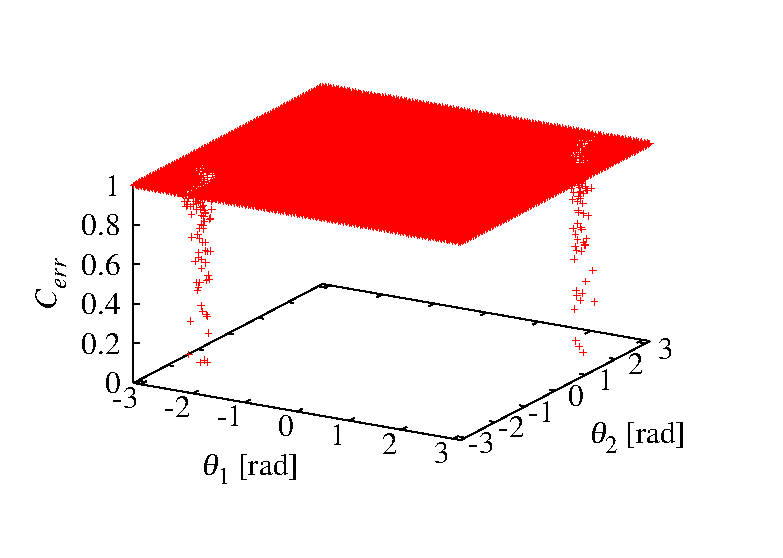
\includegraphics[width=1.0\linewidth]{fig/energy/analysis/err.eps}
  \end{minipage}
  \begin{minipage}{0.37\linewidth}
    \centering
    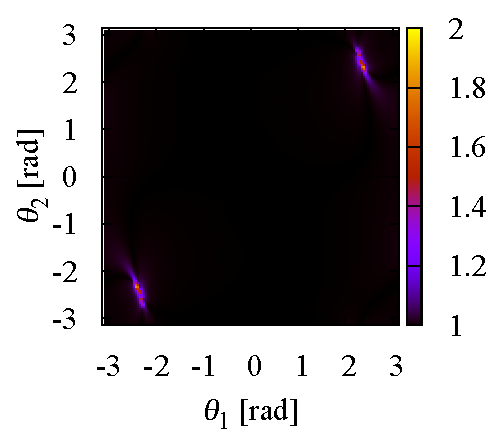
\includegraphics[width=1.0\linewidth]{fig/energy/analysis/err_2d.eps}
  \end{minipage}
  \caption{The distribution of the cost function with the two-DoF model.}
  \label{fig:dist_2D}
\end{figure}
% ---------------------------------------------------------------------
%
From the result,
we can confirm that $C_{ratio} \approx 1$ at almost all points.
Indeed, the average of $C_{ratio}$ is $1.002$ among all points.
Hence, these motions are equivalent in this model.
Here, we should note that there are large errors in specific points.
This non-correspondence will be discussed below.



%%%%%%%%%%%%%%%%%%%%%%%%%%%%%%%%%%%%%%%%%%%%%%%%%%%%%%%%%%
\subsubsection{Influence arising from parameters variation}
%%%%%%%%%%%%%%%%%%%%%%%%%%%%%%%%%%%%%%%%%%%%%%%%%%%%%%%%%%
Before discussing spatial model,
we should identify the influence arising from parameter variation.
Here, we focus on total link mass and the CoM position of each link according to the following equation:
%
% ---------------------------------------------------------------------
\begin{align}
  m_{i}^{*} &= \alpha m_{i}\\
  l^{*}_{ci} &= \beta l_{ci}
\end{align}
% ---------------------------------------------------------------------
%
where, $0.5 \leq \alpha \leq 1.5$,
$0.5 \leq \beta \leq 1.5$ are scaling factors,
$m_{i}$,
$l_{ci} = l_{i}/2$ are the original mass and length to the CoM position of each link as explained above ($m_{i} = 100\unit{kg}$, $l_{i} = 1\unit{m}$).
$(\circ)^{*}$ denotes the modified parameter.
%
% ---------------------------------------------------------------------
\begin{figure}[t]
  \centering
  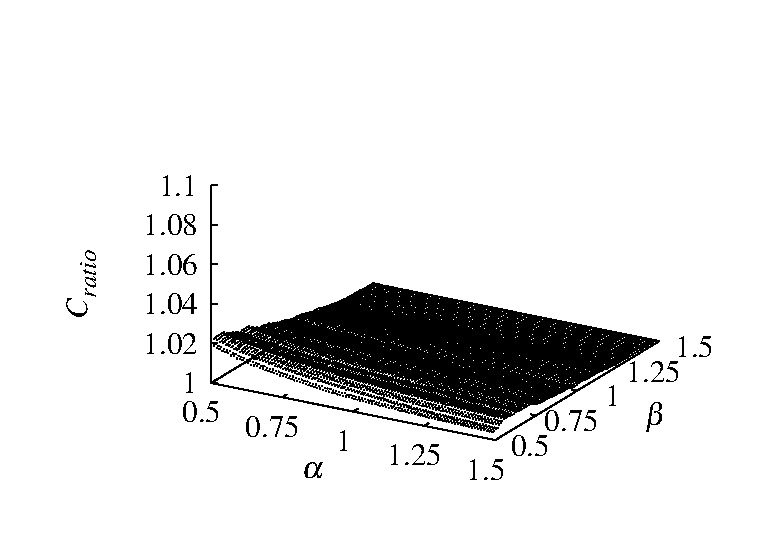
\includegraphics[width=0.6\linewidth]{fig/energy/analysis/parameter.eps}
  \vspace{-2em}
  \caption{This figure shows how the average of $C_{ratio}$ is affected by parameter variation.}
  \label{fig:parameter}
\end{figure}
% ---------------------------------------------------------------------
%
Average of $C_{ratio}$ under the parameter variation is displayed in \fig{parameter}.
This figure shows that reactionless motion coincides
with instantaneous minimum motion even if parameters are changed.
In particular, high equivalence can be observed when $\alpha$ takes large values.



%%%%%%%%%%%%%%%%%%%%%%%%%%%%%%%%%%%%%%%%%%%%%%%%%%%%
\subsubsection{Four-DoF spatial manipulator}
%%%%%%%%%%%%%%%%%%%%%%%%%%%%%%%%%%%%%%%%%%%%%%%%%%%%
Here, we identify the equivalence with a four-DoF spatial manipulator.
As the our manipulator model, the positioning subchain of the seven-DoF redundant manipulator is considered.
The reaction wheel parameters are same as one which was used in the planar case.
In this case, the same cost function is also used to evaluate the equivalence.
The calculation range is as follows:
%
% ---------------------------------------------------------------------
\begin{align}
  &-\pi \leq \theta_{i} \leq \pi\notag\\
  &\Delta \theta_{i} = 0.125\unit{rad}~(i = 1,3,4)\\
  &-\frac{\pi}{2} \leq \theta_{2} \leq \frac{\pi}{2}\notag\\
  &\Delta \theta_{2} = 0.0628\unit{rad}
\end{align}
% ---------------------------------------------------------------------
%
where, we restrict the range of joint 2 because almost all configurations over the above range
have no meaning due to the collision with the satellite.
Totally, the cost function is calculated at $6.25\times 10^{6}$ points.

Because of too many parameters to draw graph,
we show the distribution of $C_{ratio}$ parametrized for joint 1 and 2.
First, we show a distribution map which does not include large errors in \fig{dist_3d}~(a).
The map was obtained with parametrized for $(\theta_{1}, \theta_{2}) = (-3.05,0.403)\unit{rad}$.
Except few configurations,
reactionless motion coincides the energy minimum motion as seen in the planar case.
However, we observe inconsistency with specific configurations.
An example is shown in \fig{dist_3d}~(b) with parametrized for $(\theta_{1},\theta_{2}) = (-\pi,0)\unit{rad}$.
Despite these large errors,
the average value of $C_{ratio}$ is $1.14$.
Hence, reactionless motion produces almost minimum energy.
In what follows, we discuss the reason of the equivalence and the inconsistency.
%
% ---------------------------------------------------------------------
\begin{figure}[t]
  \centering
  \begin{minipage}[t]{0.495\linewidth}
    \centering
    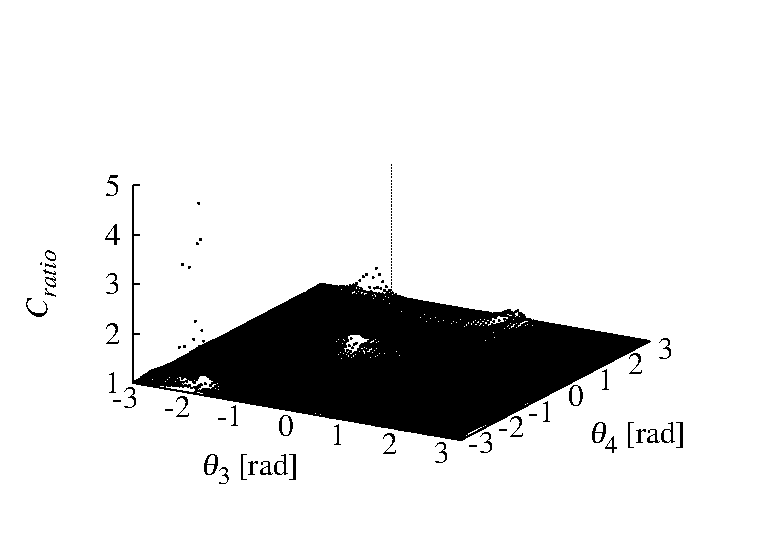
\includegraphics[width=1.0\linewidth]{fig/energy/analysis/err-3.05183_0.403919.eps}
    \footnotesize\par{(a)}
  \end{minipage}
  \begin{minipage}[t]{0.495\linewidth}
    \centering
    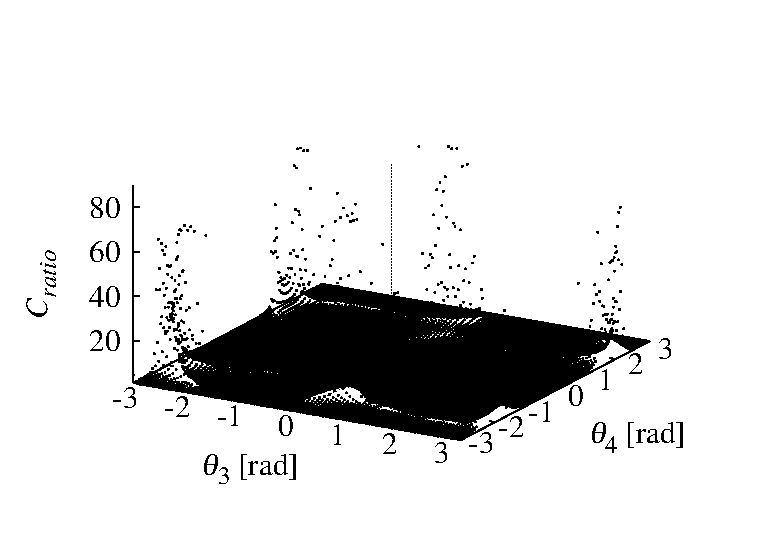
\includegraphics[width=1.0\linewidth]{fig/energy/analysis/err-3.14159_0.eps}
    \footnotesize\par{(b)}
  \end{minipage}
  \caption{The disutribution of cost function with the four-DoF spatial manipulator model:
  (a) regularly appearing distribution $(\theta_{1},\theta_{2}) = (-3.05,0.403)\unit{rad}$
  and (b) near the singularity $(\theta_{1},\theta_{2}) = (-\pi,0)\unit{rad}$.}
\label{fig:dist_3d}
\end{figure}
% ---------------------------------------------------------------------
%

%%%%%%%%%%%%%%%%%%%%%%%%%%%%%%%%%%%%%%%%%%%%%%%%%%%%%%%%%%%%%%
\subsubsection{Discussion about the equivalence}
\label{sec:DISCUSS}
%%%%%%%%%%%%%%%%%%%%%%%%%%%%%%%%%%%%%%%%%%%%%%%%%%%%%%%%%%%%%%
Here, we discuss why these motions are equivalent.
To answer the question, we should identify a property of kinetic energy 
produced by both manipulator and reaction wheels under zero base-attitude deviation.
This property appears in the inertia matrix.
$\hat{\bm{M}}_{m}$ and
$\hat{\bm{M}}_{r}$ are rewritten in the following form:
%
% ---------------------------------------------------------------------
\begin{align}
  \hat{\bm{M}}_{m} = &\sum_{i=1}^{n}\Big\{m_{i}\bm{J}_{vi}^{T}\bm{J}_{vi} + \bm{J}_{\omega i}^{T}\bm{I}_{i}\bm{J}_{\omega i}\Big\}\label{eq:mani}\\
  \hat{\bm{M}}_{r} = &\frac{1}{I_{r}}\sum_{i=1}^{n}\Big\{m_{i}^{2}\bm{J}_{v i}^{T}\bm{r}_{i}^{\times}{}^{T}\bm{r}_{i}^{\times}\bm{J}_{vi}+
\bm{J}^{T}_{\omega i}\bm{I}_{i}\bm{I}_{i}\bm{J}_{\omega i} +\notag\\
  &m_{i}\bm{J}_{\omega i}^{T}\bm{I}_{i}\bm{r}_{i}^{\times}\bm{J}_{vi} + [ m_{i}\bm{J}_{\omega i}^{T}\bm{I}_{i}\bm{r}_{i}^{\times}\bm{J}_{vi}]^{T}\Big\}\label{eq:rw}
\end{align}
% ---------------------------------------------------------------------
%
where, $m_{i}$, $\bm{I}_{i}\R{3}$ are $i$th link mass and inertia tensor,
$\bm{J}_{vi}$,
$\bm{J}_{\omega i}\R{3 \times n}$ stand for the Jacobian w.r.t.\ linear and angular velocity of each link,
$\bm{r}_{i}\R{3}$ is the position vector of $i$th link CoM w.r.t.\ the base CoM.
Here, we assume general $n$-link manipulator model.
Note that base linear motion related terms are ignored for the sake of simplicity.

From \eq{mani},
it can be seen that the kinetic energy induced by the manipulator motion is represented
as a linear function in terms of the inertia parameters of manipulator.
On the other hand,
reaction wheel related energy is a quadratic function in terms of same parameters;
it is also proportion to the inverse of the inertia moment of the reaction wheel,
which is usually enough smaller than 1.
Hence, we can conclude that the reaction wheel producing kinetic energy is far larger than the manipulator's one.
This feature would make reactionless motion potentially effective in terms of energy consumption because no usage of
reaction wheels.

On the other hand,
compared with the results in \fig{BIF_VEC}~(b) and \fig{dist_2D},
we can find that the inconsistency happens around the singularity of the coupling inertia matrix.
In particular, at the singular configuration,
any motion does not disturb the base attitude
because the null-space of the coupling inertia matrix
coincides with the tangential space of joint space $T_{\theta}(\mathbb{R}^{2})$:
namely an additional reactionless motion vector appears at the singularity.
In this case, reactionless motion must be energy minimum.
On the other hand,
near the singularities,
reactionless motion does not coincide with the instantaneous energy minimum motion, in general.
Since the base disturbance is quite small near the singularity:
e.g.\ reaction wheel is hardly needed,
reactionless motion can be different from the minimum energy one.


%%%%%%%%%%%%%%%%%%%%%%%%%%%%%%%%%%%%%%%%%%%%%%%%
\subsection{Comparison study under the inspection task}
\label{sec:comp}
%%%%%%%%%%%%%%%%%%%%%%%%%%%%%%%%%%%%%%%%%%%%%%%%

%%%%%%%%%%%%%%%%%%%%%%%%%%%%%%%%%%%%%
\subsubsection{Simulation condition}
%%%%%%%%%%%%%%%%%%%%%%%%%%%%%%%%%%%%%
Finally, we evaluate the performance of using reactionless motion control in terms of energy consumption
at the inspection maneuver.
From the above analysis, reactionless motion is nearly energy minimum and
reaction wheels are needed a large energy to compensate a base disturbance.

We consider the following cost functions to evaluate the performance:
%
% ---------------------------------------------------------------------
\begin{align}
  C_{max} &= \frac{1}{2}\max_{t_{0} \leq t \leq t_{f}}\Big(\thd^{T}(t)\hat{\bm{M}}\thd(t)\Big)\label{eq:Tmax}\\
  C_{sum} &= \frac{1}{2}\int_{t_{0}}^{t_{f}}\thd^{T}(t)\hat{\bm{M}}\thd(t)dt\label{eq:Tsum}
\end{align}
% ---------------------------------------------------------------------
%
% \eq{Tmax} is the maximum kinetic energy,
% \eq{Tsum} expresses the whole kinetic energy throughout the motion tasks.

In order to realize zero base-attitude deviation with reaction wheels,
the reaction wheel torque must ensure the following condition:
%
% ---------------------------------------------------------------------
\begin{align}
  \bm{\tau}_{r}^{ref} = -\frac{d}{dt}(\tbm{M}_{\omega m}\thd^{ref}(t))
\end{align}
% ---------------------------------------------------------------------
%
where, $\thd^{ref}$ is the pre-defined reference control command for the manipulator.

We compare the above costs under the camera inspection task under five conditions
with some initial configurations and the desired motions.
At all of them, simulation time is set as $20\unit{s}$ and the comparison controller is
the inverse Jacobian controller using only the wrist assembly as explained in the previous section.


%%%%%%%%%%%%%%%%%%%%%%%%%%%%%%%%%%
\subsubsection{Simulation results}
%%%%%%%%%%%%%%%%%%%%%%%%%%%%%%%%%%
%
% ---------------------------------------------------------------------
\begin{figure}[t]
  \centering
  \begin{minipage}[h]{0.5\linewidth}
    \centering
    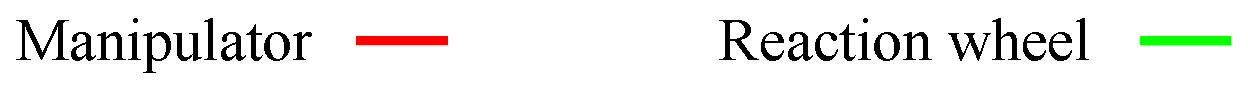
\includegraphics[width=1.0\linewidth]{fig/energy/comparison/energy.eps}
  \end{minipage}\\
  \vspace{-4mm}
  \begin{minipage}[h]{0.40\linewidth}
    \centering
    \includegraphics[width=1.0\linewidth]{fig/energy/comparison/RL-M/RNS_U10_partial_kinetic_energy.eps}
  \end{minipage}
  \hspace{-4mm}
  \begin{minipage}[h]{0.40\linewidth}
    \centering
    \includegraphics[width=1.0\linewidth]{fig/energy/comparison/RW-M/RNS_U10_partial_kinetic_energy.eps}
  \end{minipage}\\
  \vspace{-7mm}
  \centering
  \begin{minipage}[h]{0.350\linewidth}
    \centering
    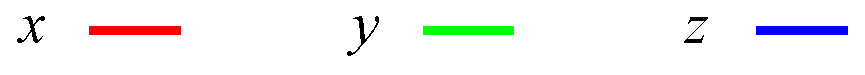
\includegraphics[width=1.0\linewidth]{fig/energy/comparison/torque.eps}
  \end{minipage}\\
  \vspace{-4mm}
  \begin{minipage}[h]{0.40\linewidth}
    \centering
    \includegraphics[width=1.0\linewidth]{fig/energy/comparison/RL-M/RNS_U03_reaction_wheel_torque.eps}
    \footnotesize\par{\vspace{-2mm}\hspace{8mm}Reactionless}
  \end{minipage}
  \hspace{-4mm}
  \begin{minipage}[h]{0.40\linewidth}
    \centering
    \includegraphics[width=1.0\linewidth]{fig/energy/comparison/RW-M/RNS_U03_reaction_wheel_torque.eps}
    \footnotesize\par{\vspace{-2mm}\hspace{8mm}Reaction wheel used}
  \end{minipage}\\
  \vspace{-4mm}
  \vspace{1em}
  \caption{An example of energy consumption comparison.}
  \label{fig:RES_ENE}
\end{figure}
% ---------------------------------------------------------------------
%
First, we show an example.
The conditions were same as ones which were considered in \sec{PROPOSAL} (the case of \fig{ins}~(a)).
The results are displayed in \fig{RES_ENE}.
% In the graphs, we use log scale to display kinetic energy both the manipulator and the reaction wheel.
We can see that the kinetic energy produced by the reaction wheel is quite larger than
that by the manipulator motion.
As a result, reactionless motion control has an advantage in terms of energy consumption
as described above.
In addition,
if we plan to perform this inspection task with reaction wheels,
the manipulator has to be driven at lower speed because the limitation of the reaction wheel torque
general poor:
the limitation is $0.1\unit{Nm}$ in the ETS-VII.

Next we compare the cost over five conditions.
The results are displayed with bar graph in \fig{RES_ENE_COMP}.
The red bar expresses the result under reactionless motion control;
the green bar is that with the reaction wheels.
Note that the axis of kinetic energy is represented as log scale.
From the results,
it can be seen that energy consumption under reactionless motion is also quite smaller than that of
the reaction wheel based method.
Actually, almost $10^{3}$ times reduction is observed in the both cost functions.
This result is due to the large energy consumption of reaction wheel as explained in \eq{rw}.
In summary, we can conclude that energy consumption can be largely reduced in addition to mission duration,
by using reactionless motion control.

%
% ---------------------------------------------------------------------
\begin{figure}[t]
  \centering
  \begin{minipage}[t]{0.47\linewidth}
    \centering
    \includegraphics[width=1.0\linewidth]{fig/energy/comparison/comp.eps}
  \end{minipage}\\
  \vspace{-2mm}
  \begin{minipage}[t]{0.45\linewidth}
    \centering
    \includegraphics[width=1.0\linewidth]{fig/energy/comparison/01_maximum.eps}
  \end{minipage}
  \hspace{-4mm}
  \begin{minipage}[t]{0.45\linewidth}
    \centering
    \includegraphics[width=1.0\linewidth]{fig/energy/comparison/02_integral.eps}
  \end{minipage}
  \caption{Comparison of energy consumption under five conditions}
  \label{fig:RES_ENE_COMP}
\end{figure}
% ---------------------------------------------------------------------
%


%%%%%%%%%%%%%%%%%%%%%%%%%%%%%%%%%%%%%%%%%%%%%%%%
\section{Conclusion}
\label{sec:CON}
%%%%%%%%%%%%%%%%%%%%%%%%%%%%%%%%%%%%%%%%%%%%%%%%
In this work, we tackled the following three issues in reactionless motion control.
(i) motion analysis of reactionless control
(ii) proposal of a motion task suitable for execution under reactionless motion control
and
(iii) energy consumption under zero base-attitude deviation.

Despite some researchers have addressed reactionless motion control,
reactionless motion itself seems to be unclear.
We analyzed reactionless motion with a planar two-DoF model through numerical calculation.
From the result, we show a new character of reactionless motion.
Among its model parameters, the manipulator attachment position plays an important role as
a bifurcation parameter.
When a displacement between the base CoM and the manipulator attachment position is large,
occurrence of fixed points/singularities was observed.
If we plan to use reactionless motion control,
this character should be included with manipulator designs.
This design issue for reactionless motion will be considered as the future task.

On the other hand,
as a practical use of reactionless motion,
we proposed an inspection task using a hand camera with a seven-DoF redundant manipulator.
With this model, its reactionless motion is approximately represented a superposition between
predominant wrist and elbow motion.
Based on the predominant wrist motion,
we designed a controller for inspection task based on the theory of task priority.
The base attitude (reactionless) constraint was considered as the primary task;
the end-effector orientation control is the second one;
the wrist position stabilization was performed as the third priority.
From the verification via numerical simulations,
we showed this reactionless task can be useful compared with the traditional inverse Jacobian controller.
In addition,
we showed the effectiveness of the damped least-squares inverse to the algorithmic singularity within
the end-effector reactionless control.

Finally, we discussed energy consumption under zero base-attitude deviation.
We evaluated the performance of energy consumption with kinetic energy produced by
both the manipulator and reaction wheels.
Mathematically, the kinetic energy of reaction wheel is represented as
a quadratic function of the parameters of the manipulator,
while the kinetic energy of the manipulator is a linear function of the parameters.
This feature makes reactionless motion effectiveness in terms of energy consumption.
Indeed, reactionless motion produces almost minimum energy.
Under the inspection maneuver, we verified the energy consumption of reactionless motion
compared with a reaction wheel based reaction compensation.
As a result,
$10^{3}$ times reduction of energy consumption can be observed using reactionless motion.


%%%%%%%%%%%%%%%%%%%%%%%%%%%%%%%%%%%%%%%%%%%%%%%%
% Reference
\bibliographystyle{elsarticle-num}
\bibliography{bibitem}
%%%%%%%%%%%%%%%%%%%%%%%%%%%%%%%%%%%%%%%%%%%%%%%%

\end{document}
\endinput
%%
%% End of file `elsarticle-template-num.tex'.
